% -*- Mode: Latex; -*-
% ------------------------------------------------------------------------
% Default style
% ------------------------------------------------------------------------

\documentclass[11pt]{article}
\usepackage[numbers]{natbib}
\usepackage{macros/packages}
\usepackage{macros/editing-macros}
\usepackage{macros/formatting}
\usepackage{macros/statistics-macros}
\usepackage[utf8]{inputenc} % allow utf-8 input
\usepackage[T1]{fontenc}    % use 8-bit T1 fonts
\usepackage{hyperref}       % hyperlinks
\usepackage{url}            % simple URL typesetting
\usepackage{booktabs}       % professional-quality tables
\usepackage{amsfonts}       % blackboard math symbols
\usepackage{nicefrac}       % compact symbols for 1/2, etc.
\usepackage{microtype}      % microtypography
\usepackage{xcolor}         % colors
\usepackage{wrapfig}
\usepackage{subcaption}
\usepackage{tikz}
\usetikzlibrary{%
  calc,
  fit,
  arrows,
  arrows.meta,
  positioning,
  decorations.pathreplacing,
  decorations.shapes,
}

% \onehalfspacing
% \renewcommand{\baselinestretch}{1.35}

\begin{document}

% Control whitespace around equations
\abovedisplayskip=8pt plus0pt minus3pt
\belowdisplayskip=8pt plus0pt minus3pt

% ------------------------------------------------------------------------
% Main Paper Body
% ------------------------------------------------------------------------


% ------------------------------------------------------------------------
% Default title and authorship
% ------------------------------------------------------------------------
\begin{center}
  {\huge PersonalLLM: Tailoring LLMs to Individual Preferences } \\
  \vspace{.5cm} {\Large Thomas P. Zollo$^*$ ~~~ Andrew Siah$^*$}\footnote{* These authors contributed equally to this work}\\
  
  \vspace{.2cm}
  {\Large ~~~ Naimeng Ye ~~ Ang Li ~~ Hongseok Namkoong} \\
  \vspace{.2cm}
  {\large Columbia University} \\
  \vspace{.2cm}
  \texttt{\{tpz2105, andrew.siah, ny2336, al4263, hongseok.namkoong\}@columbia.edu}
\end{center}



% ------------------------------------------------------------------------
% Abstract
% ------------------------------------------------------------------------




\begin{abstract}

As LLMs become capable of complex tasks, there is growing potential for personalized interactions tailored to the subtle and idiosyncratic preferences of the user.
We present a public benchmark, PersonalLLM, focusing on adapting LLMs to provide maximal benefits for a particular user. 
Departing from existing alignment benchmarks that implicitly assume uniform preferences, we curate open-ended prompts paired with many high-quality answers over which users would be expected to display heterogeneous latent preferences.
Instead of persona prompting LLMs based on high-level attributes (e.g., user race or response length), which yields homogeneous preferences relative to humans, we develop a method that can simulate diverse preferences from a set of pre-trained reward models.
Our dataset and generated personalities offer an innovative testbed for developing personalization algorithms that grapple with continual data sparsity---few relevant feedback from the particular user---by leveraging historical data from other (similar) users.
We explore basic in-context learning and meta-learning baselines to illustrate the utility of PersonalLLM and highlight the need for future methodological development.

\end{abstract}


\section{Introduction}

The \textit{alignment} of LLMs with human preferences has recently 
received much attention, with a focus on adapting model outputs to reflect universal population-level values.
A typical goal is to take a pre-trained model that cannot reliably follow complex user instructions \citep{wei2022finetuned} and can easily be made to produce dangerous and offensive responses \citep{perez2022red},
and adapt it to  the instructions of its user base \citep{ouyang2022training} or train a generally helpful and harmless assistant \citep{bai2022training}. 
By assuming a \emph{uniform preference} across the population, recent successes~\citep{ziegler2020finetuning, ouyang2022training, christiano2023deep} demonstrate the feasibility of learning
and optimizing a monolithic preference (``reward model''). Alignment techniques have provided the basis for popular commercial applications like ChatGPT, as well as instruction-tuned open-source models \citep{touvron2023llama}.

The rapid advancement in LLM capabilities opens the door to an even more refined notion of human preference alignment: personalization.
A personalized model should adapt to the preferences and needs of a particular user, and provide maximal benefits as it accumulates interactions (see Figure~\ref{fig:main_figure}).
Given the expected data sparsity in this setting, beyond a particular user's data, such personalized language systems will likely also rely on historical data from other (similar) users in order to learn how to learn from a small set of new user feedback (see Figure~\ref{fig:metalearn}).
By discovering patterns across users, these systems will be able to efficiently optimize their responses, ultimately leading to more effective and beneficial conversational AI.  For example:
\begin{itemize}
\item A personalized learning experiences could be crafted by adapting educational chat assistants to the specific learning pace and style of individual students based on previous successful interactions with similar students.  
\item 
Customer support chatbots could offer more accurate and empathetic responses by drawing on a wealth of previous interactions, leading to quicker resolution times and higher customer satisfaction. 
\item In healthcare, personalized chatbots could provide tailored advice based on patients with similar medical history and communication preferences. 
\end{itemize}

Compared to conventional applications where prompts have a uniform notion of ``ground truth'' (e.g., question answering),
LLM personalization is distinguished by the need to study open-ended prompts where users exhibit heterogeneous preferences across many possible high-quality answers.
While personal preferences may vary according to simple features like user age \cite{chan2024scalingsyntheticdatacreation, castricato2024personareproducibletestbedpluralistic} and answer length and technicality \cite{li2024personalizedlanguagemodelingpersonalized}, they also involve more abstract dimensions of culture, politics, and language \cite{kirk2024prismalignmentprojectparticipatory}, as well as aspects of personality that are difficult to explain \citep{hwang2023aligninglanguagemodelsuser}.
A personalized LLM should be able to adapt to 
subtle, idiosyncratic, and sometimes sensitive differences between user tastes as it gathers more interactions.

\begin{figure}[t]
    \centering
    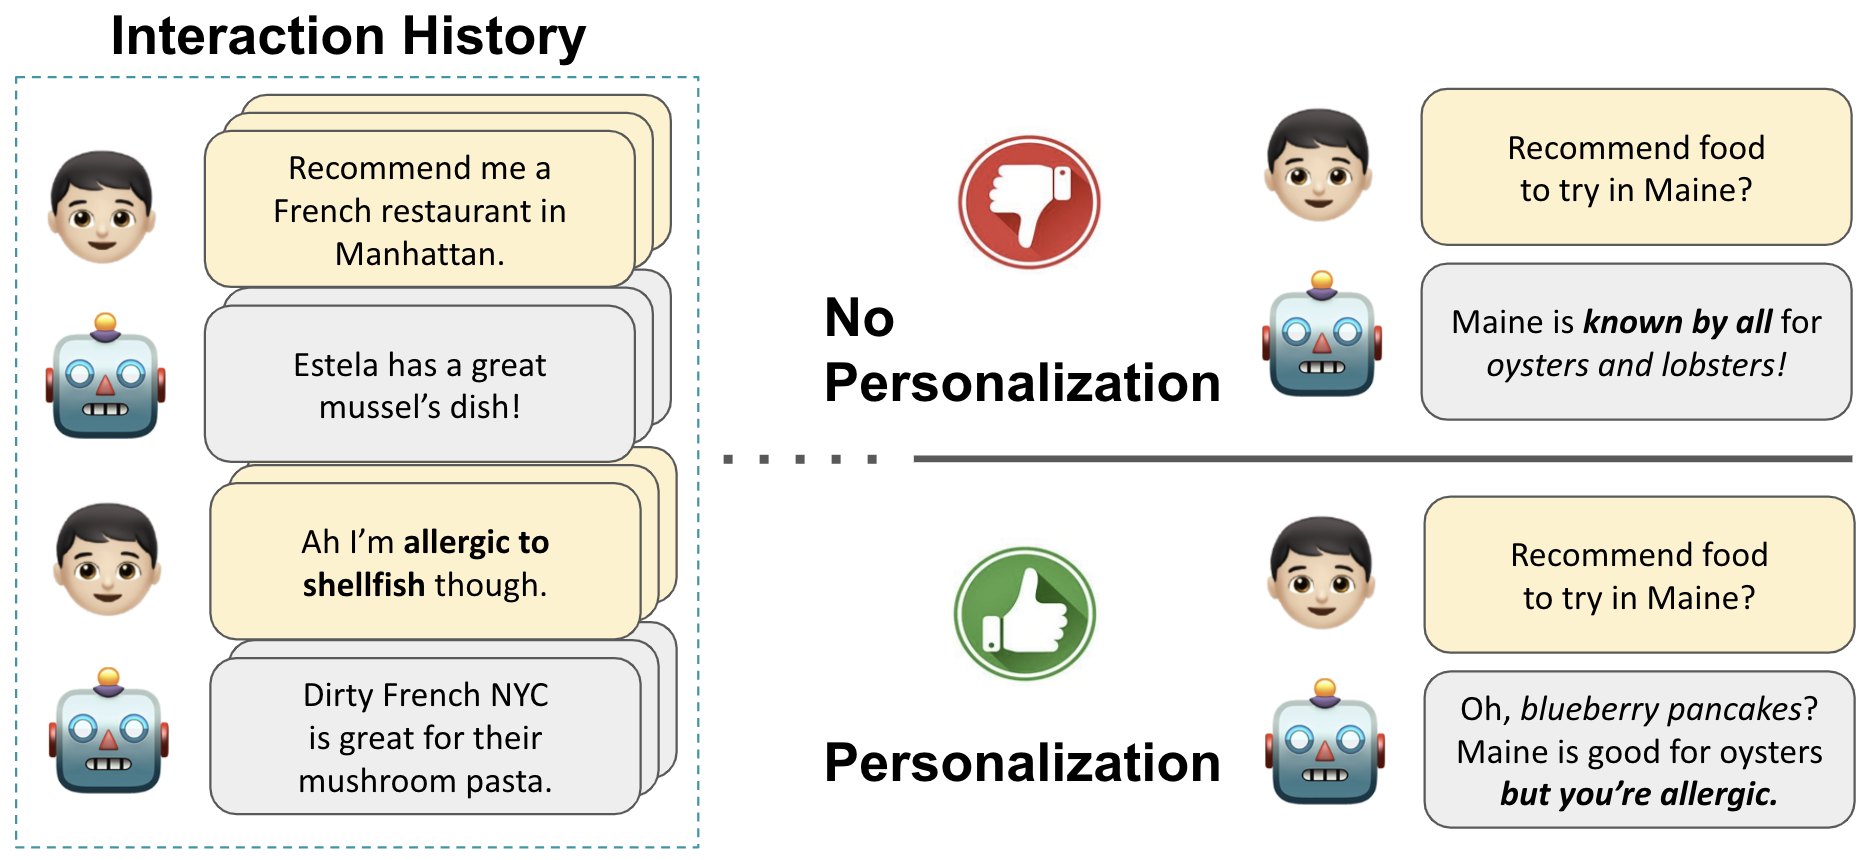
\includegraphics[width=\textwidth]{../figures/fig1.png}
    \caption{
    Standard LLMs require tedious re-prompting to learn a user’s preferences in each session. \textsf{PersonalLLM} aims to learn a unique user's diverse preferences to maximize long-term satisfaction.}
    \label{fig:main_figure}
\end{figure}

Inspired by the vision of a future with personalized AI, we introduce \textsf{PersonalLLM}, a public, open-source benchmark designed to adapt LLMs to provide maximal benefits for individual users. In order to explore complex differences in user tastes, our benchmark features a set of prompts with many high-quality LLM responses (from state-of-the-art LLMs like GPT-4o, Claude 3 Opus, and Gemini 1.5 Pro), such that humans \textit{are expected} to express diverse preferences over the responses.
Such an approach to dataset-building stands in contrast to existing alignment datasets, where responses exhibit observable quality differences (see Figure~\ref{fig:PersonalLLM}).

For each prompt and set of responses, our dataset also includes scores from a set of 10 reward models with heterogeneous preferences over those responses.
We leverage these reward models to sample many new ``users'' (or personal preference models) via weighted ensembles of their preferences, and in doing so we are able to \textit{simulate an entire user base}, which we argue to be a critical ingredient in a truly useful personalization benchmark.  
Through extensive analysis of the preferences of these users over our dataset, we show these simulated personal preference models to be diverse and non-trivial (e.g., with respect to length, formatting, or tone). We illustrate the difficulty of creating such an environment by comparing to the increasingly popular persona prompting baseline \citep{castricato2024personareproducibletestbedpluralistic, chan2024scalingsyntheticdatacreation, jang2023personalizedsoupspersonalizedlarge}, which in our analysis produces preferences only half as diverse as a set of \textsf{PersonalLLM} users across multiple metrics.
Taken together, the prompts, responses, and personalities present in \textsf{PersonalLLM} offer an innovative tested for benchmarking personalization algorithms as they tailor interactions based on previous interactions with an individual user.

While fine-tuning and reinforcement learning approaches \citep{schulman2017proximal, rafailov2023direct} are effective for aligning to population-level preferences,
personalization requires a new algorithmic toolkit, as it is not practical to gather enough data or
store a separate copy of the model or even low-rank adapter weights \citep{Hu2021} for every user.
\textsf{PersonalLLM} offers the versatility necessary to spur development across a range of new approaches to personalization: in-context learning (ICL) \citep{brown2020language}, retrieval augmented generation (RAG) \citep{lewis2021retrievalaugmented}, ranking agents, efficient fine-tuning, and other adaptation techniques.
In our experiments, we highlight a particularly salient challenge compared to typical applications of personalization in recommendation systems: the space of “actions/responses” is prohibitively large to be able to explore based on interactions on a single user. Since this necessitates  \textit{learning across users}, we model this as a meta-learning problem where the goal is to leverage a wealth of prior interactions from historical users to tailor responses for a new user who do not have a significant interaction history (see Figure~\ref{fig:metalearn}).

Motivated by key methodological gaps in personalizing LLMs, here we summarize our contributions:
\begin{itemize}
    \item  We release a new open-source dataset with over 10K open-ended prompts paired with 8 high-quality responses from top LLMs.
    \item We propose a novel method for sampling ``users'' (i.e., personal preference models) that, unlike existing methods, creates diverse preferences and allows for the simulation of large historical user bases.
    \item We illustrate new possibilities for algorithmic development in learning \textit{across} users.
\end{itemize}

Our goal in creating the open-source \textsf{PersonalLLM} testbed is to facilitate work on methods to personalize the output of an LLM to the individual tastes of many diverse users.
We do not claim our simulated personal preference models provide a high-fidelity depiction of human behavior, but rather offer a challenging simulation environment that provides the empirical foundation for methodological innovation in capturing the complex array of human preferences that arise in practice.
As an analogy, while ImageNet \citep{russakovsky2015imagenetlargescalevisual} is noisy and synthetic---e.g., differentiating between 120 dog breeds is not a realistic vision task---it provides a challenging enough setting that methodological progress on ImageNet implies progress on real applications.
Similarly, we believe \textsf{PersonalLLM} is a reasonable initial step toward the personalization of language-based agents, building on the common reinforcement learning paradigm of benchmarking personalization algorithms with simulated rewards \citep{zhao2023kuaisimcomprehensivesimulatorrecommender, ie2019recsimconfigurablesimulationplatform}.


\begin{figure}[t]
    \centering
\textbf{}    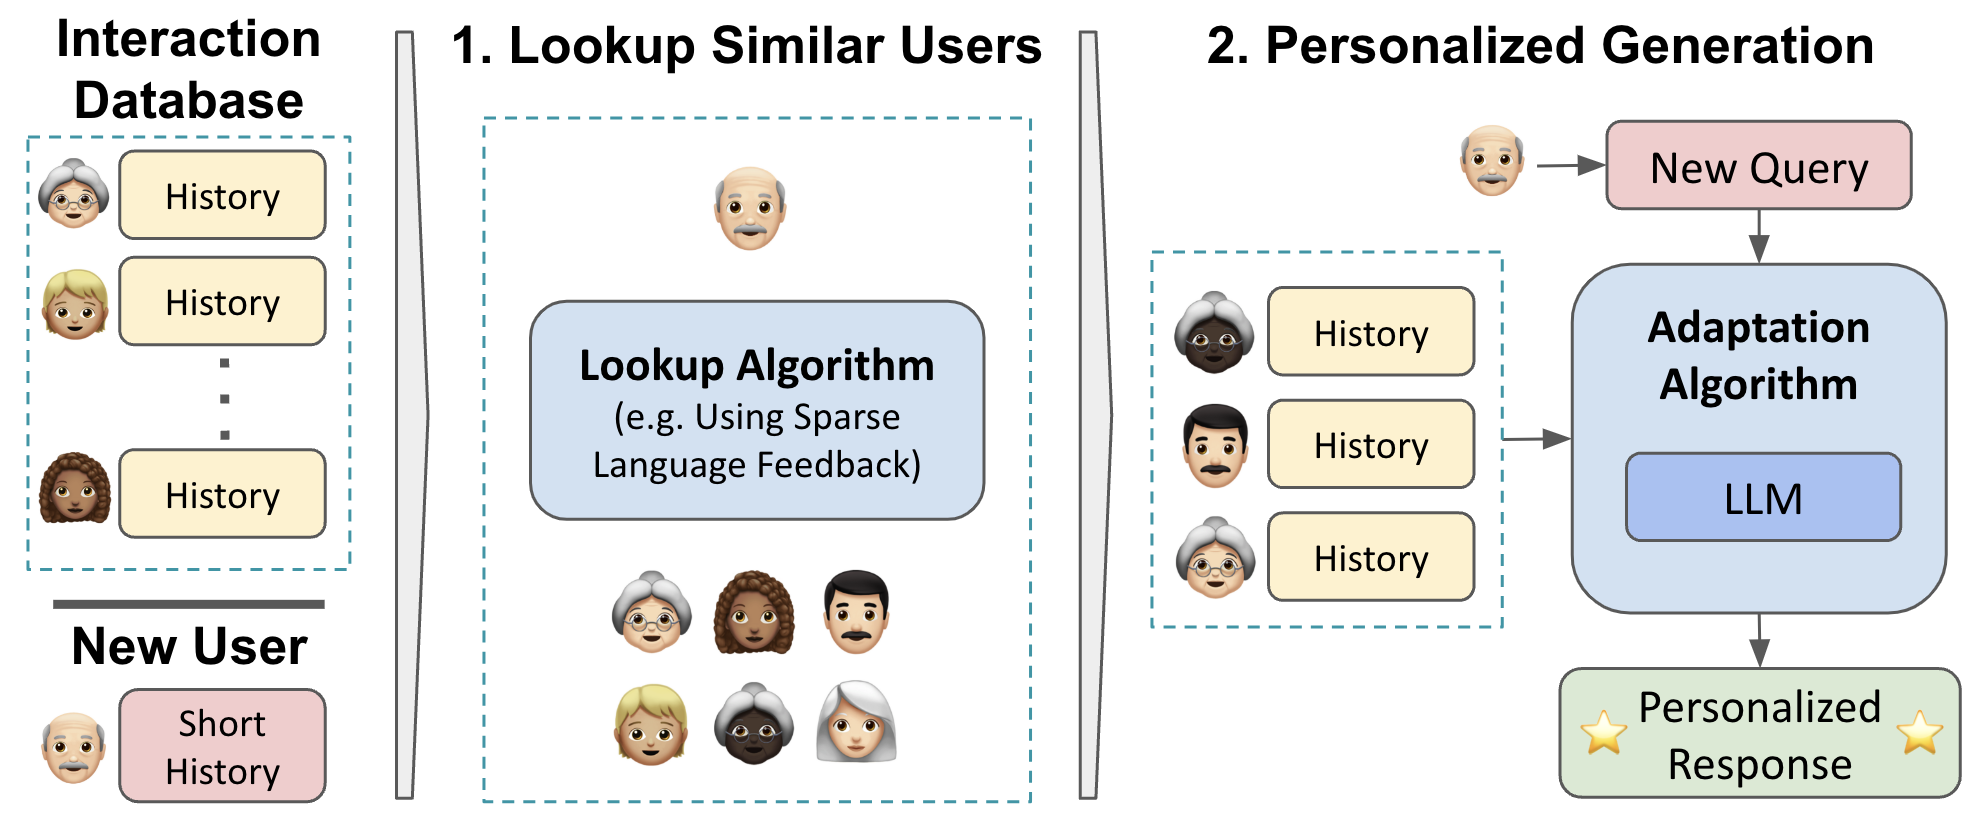
\includegraphics[width = \textwidth]{figures/metalearn_fig.png}
    \caption{In the canonical personalization setting, a dataset of historical users and their interactions is leveraged to personalize interactions for a new user with a limited history. \textsf{PersonalLLM} enables the development of such methods for learning \textit{across} users.}
    \label{fig:metalearn}
\end{figure}

\section{PersonalLLM}\label{sec:dataset}

Our \textsf{PersonalLLM} testbed is composed of two high-level components:
1) a dataset of prompts, each paired with a set of high-quality responses among which humans would be expected to display diverse preferences and
2) a method for sampling diverse personal preference models, such that we can test methods for personalization using these ``personas'' as our simulated users.
Next, we will describe each of them in detail.  Our data \footnote{\url{https://huggingface.co/datasets/namkoong-lab/PersonalLLM}} and code \footnote{\url{https://github.com/namkoong-lab/PersonalLLM}} are publicly available,  and full documentation for our dataset is available in Appendix~\ref{app:add_data_det}.

\begin{figure}[t]
    \centering
    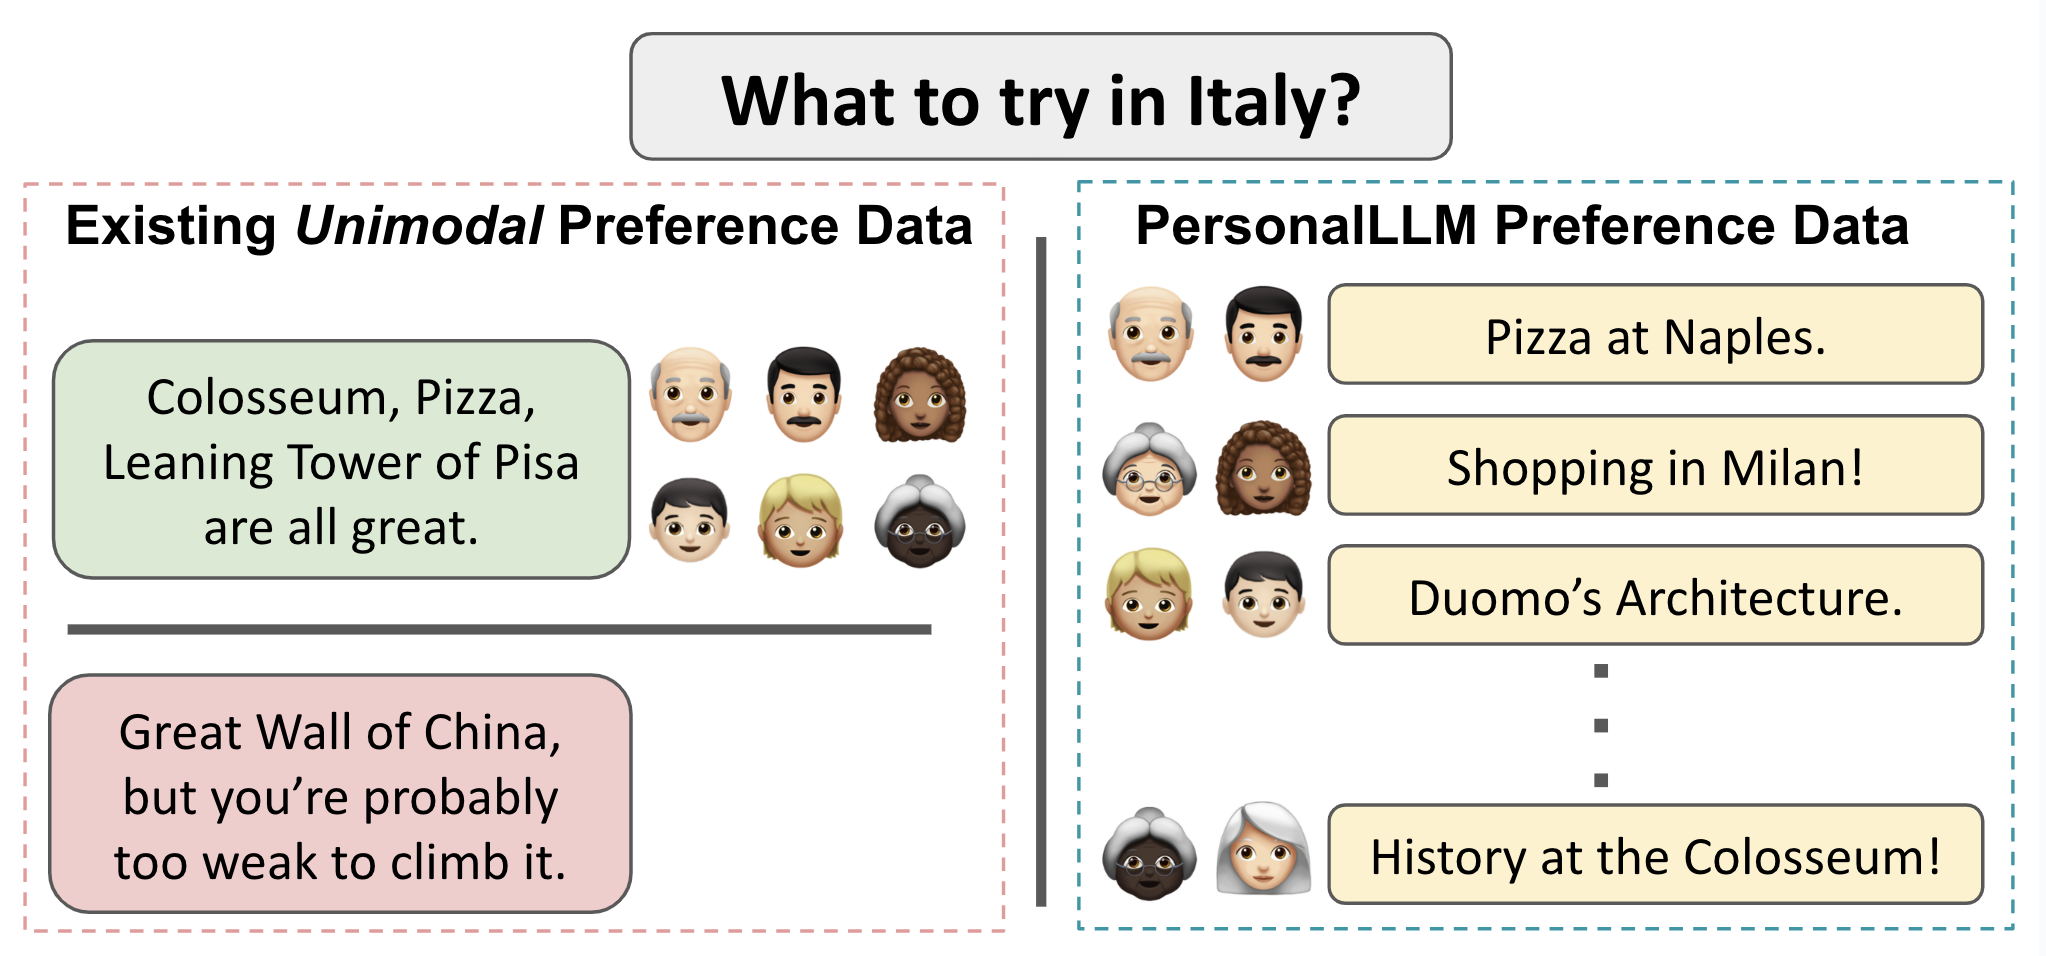
\includegraphics[width = \textwidth]{figures/data_example.png}
    \caption{\textbf{Left:} Existing alignment datasets contain prompts paired with multiple responses, where the majority of people are expected to prefer one specific response (e.g., a harmless response). \textbf{Right:} Our dataset consists of prompts paired with many high-quality responses, each favored by different personas. Such a dataset induces diverse preferences in our personal preference models, creating a testbed to build \textsf{PersonalLLM}s.}
    \label{fig:PersonalLLM}
\end{figure}

\subsection{Dataset}

Since our goal is to study diverse preferences, we first focus on collecting \textit{open-ended} prompts, similar to a chat setting.
We compile 37,919 prompts from Anthropic Helpful-online, Anthropic Helpful-base \citep{bai2022training}, Nvidia Helpsteer \citep{wang2023helpsteermultiattributehelpfulnessdataset}, and RewardBench \citep{lambert2024rewardbench}.
From this set, prompts are filtered to those with a length of 2400 characters or fewer as most reward models are limited to 4096 context length. We then randomly draw 10,402 prompts to form our final set.

Our next aim is to collect many high-quality responses for each prompt. 
Important desiderata for the generated responses are that i) they do not exhibit much variation in terms of undesirable contents (like misinformation or toxicity) or obvious dimensions of helpfulness or length, as is typical in RLHF datasets, ii) they exhibit diversity across meaningful dimensions of personal preferences like political viewpoint and culture, as well as difficult to describe latent features.
To achieve this, we generate eight responses for each of these 10,402 prompts using a selection of the top models from ChatArena and other important benchmarks: \textbf{ GPT-4o, Claude 3 Opus, Gemini-Pro-1.5, Command-R-Plus, GPT-4-Turbo, Claude 3 Sonnet, Llama3-70B-Instruct, and Mixtral 8x22B}. We split the resulting dataset into 9,402 training examples and 1,000 test examples. 

\subsection{Simulating Personal Preference Models}\label{sec:sim_users}

We design our approach to creating simulated \textsf{PersonalLLM} users with several goals in mind.
First, we aim for \textsf{PersonalLLM} to allow for the simulation of a large number of users, enabling the study of the full personalization paradigm for applications such as search engines and recommender systems \citep{davidson2010youtube, das2007google, Xu_2022, F_rber_2020} wherein a historical database of user data is leveraged to personalize new interactions.
Next, when applied to our dataset, our preference models should allow for the study of alignment based on diverse and complex latent preferences, as opposed to simple attributes such as answer length or sensitive and reductive user characteristics, for example, race or gender.
Finally, our evaluation should not rely on GPT4, which can be expensive and unsuitable for research purposes given model opacity and drift.
While human evaluation like that of \citet{kirk2024prismalignmentprojectparticipatory} is a gold standard, wherein 
fine-grained preference feedback is gathered from a representative sample of diverse and multicultural participants, it is impractical or even impossible to get this feedback throughout the methodology development cycle, meaning that synthetic personal preference models will ultimately be needed.

To overcome this difficult challenge of simulating diverse preferences, we propose a solution based on a set of strong open-source RLHF reward models.  
While it may be the case that different reward models have fairly uniform preferences over the high-quality/low-quality response pairs on which they are typically trained, we hypothesize that their preferences over many high-quality responses will instead be diverse.

Since the number of existing top-quality reward models is much smaller than the number of users we would like to simulate, we propose to generate users by sampling weightings over the set of reward models, such that the reward score assigned to a (prompt, response) pair by a user is a weighted sum of the reward scores assigned by the pre-trained reward models.
In Section~\ref{sec:persona_analysis}, we validate our hypothesis regarding the diverse and non-trivial preferences created by such sampling.

More formally, for an input prompt $x \in \mathcal{X}$, an LLM produces output response $y \in \mathcal{Y}$, where $\mathcal{X}$ and $\mathcal{Y}$ are the set of all-natural language.  Then, a preference model $\text{R}: \mathcal{X} \times \mathcal{Y} \rightarrow \mathbb{R}$ assigns a reward score to the response given to the prompt, with higher scores indicating better responses.  
Next, consider a set of $B$ base reward models, denoted as $\text{RM}_b$, $b=1,\dots,B$, and a set of $k$ $B$-\text{dimensional} weightings, which represent a set of personal preference models.  
The preference model corresponding to user $i$ can then be defined by a weighted average of these $B$ base models $\text{RM}_1, \text{RM}_2,\dots, \text{RM}_{B}$, with weights $w_1, w_2,\dots, w_B$:
\begin{align}
\vspace{-3pt}
    \text{R}^i(x,y) = \sum_{b=1}^{B} w^i_{b}\cdot\text{RM}_b(x,y)
\vspace{-3pt}
\end{align}
For our base reward models $\{\text{RM}_b\}_{b=1}^B$, we select 10 reward models with strong performance on RewardBench, an open-source benchmark for evaluating reward models.  
These reward models are built on top of popular base models such as Llama3, Mistral, and Gemma (see Appendix~\ref{app:add_data_det}).  
We evaluate each (prompt, response) pair in the train and test set with each model so that for any personality created in this manner, each (prompt, response) pair in the dataset can be scored via a simple weighting.

Taken together, our dataset and personal preference models provide an innovative and challenging environment in which to develop personalization methodology, extending the existing paradigm of simulated rewards for domains like recommender systems \citep{zhao2023kuaisimcomprehensivesimulatorrecommender, ie2019recsimconfigurablesimulationplatform} to the task of LLM personalization.

\subsubsection{Sampling User Weightings}
There are many valid ways to sample the $B$-dimensional weighting vectors.  As a simple starting point, we propose to sample from a Dirichlet distribution with a uniform concentration parameter across all classes ($w \sim \text{Dirichlet}(\alpha)$).  
As $\alpha$ becomes very small, the preference models converge towards the 10 base reward models; as it becomes large, preferences become unimodal.  Such a parameter allows us to simulate user bases with different underlying preference structures, as we detail in the next section.




\begin{figure}[!ht]
    \centering 
    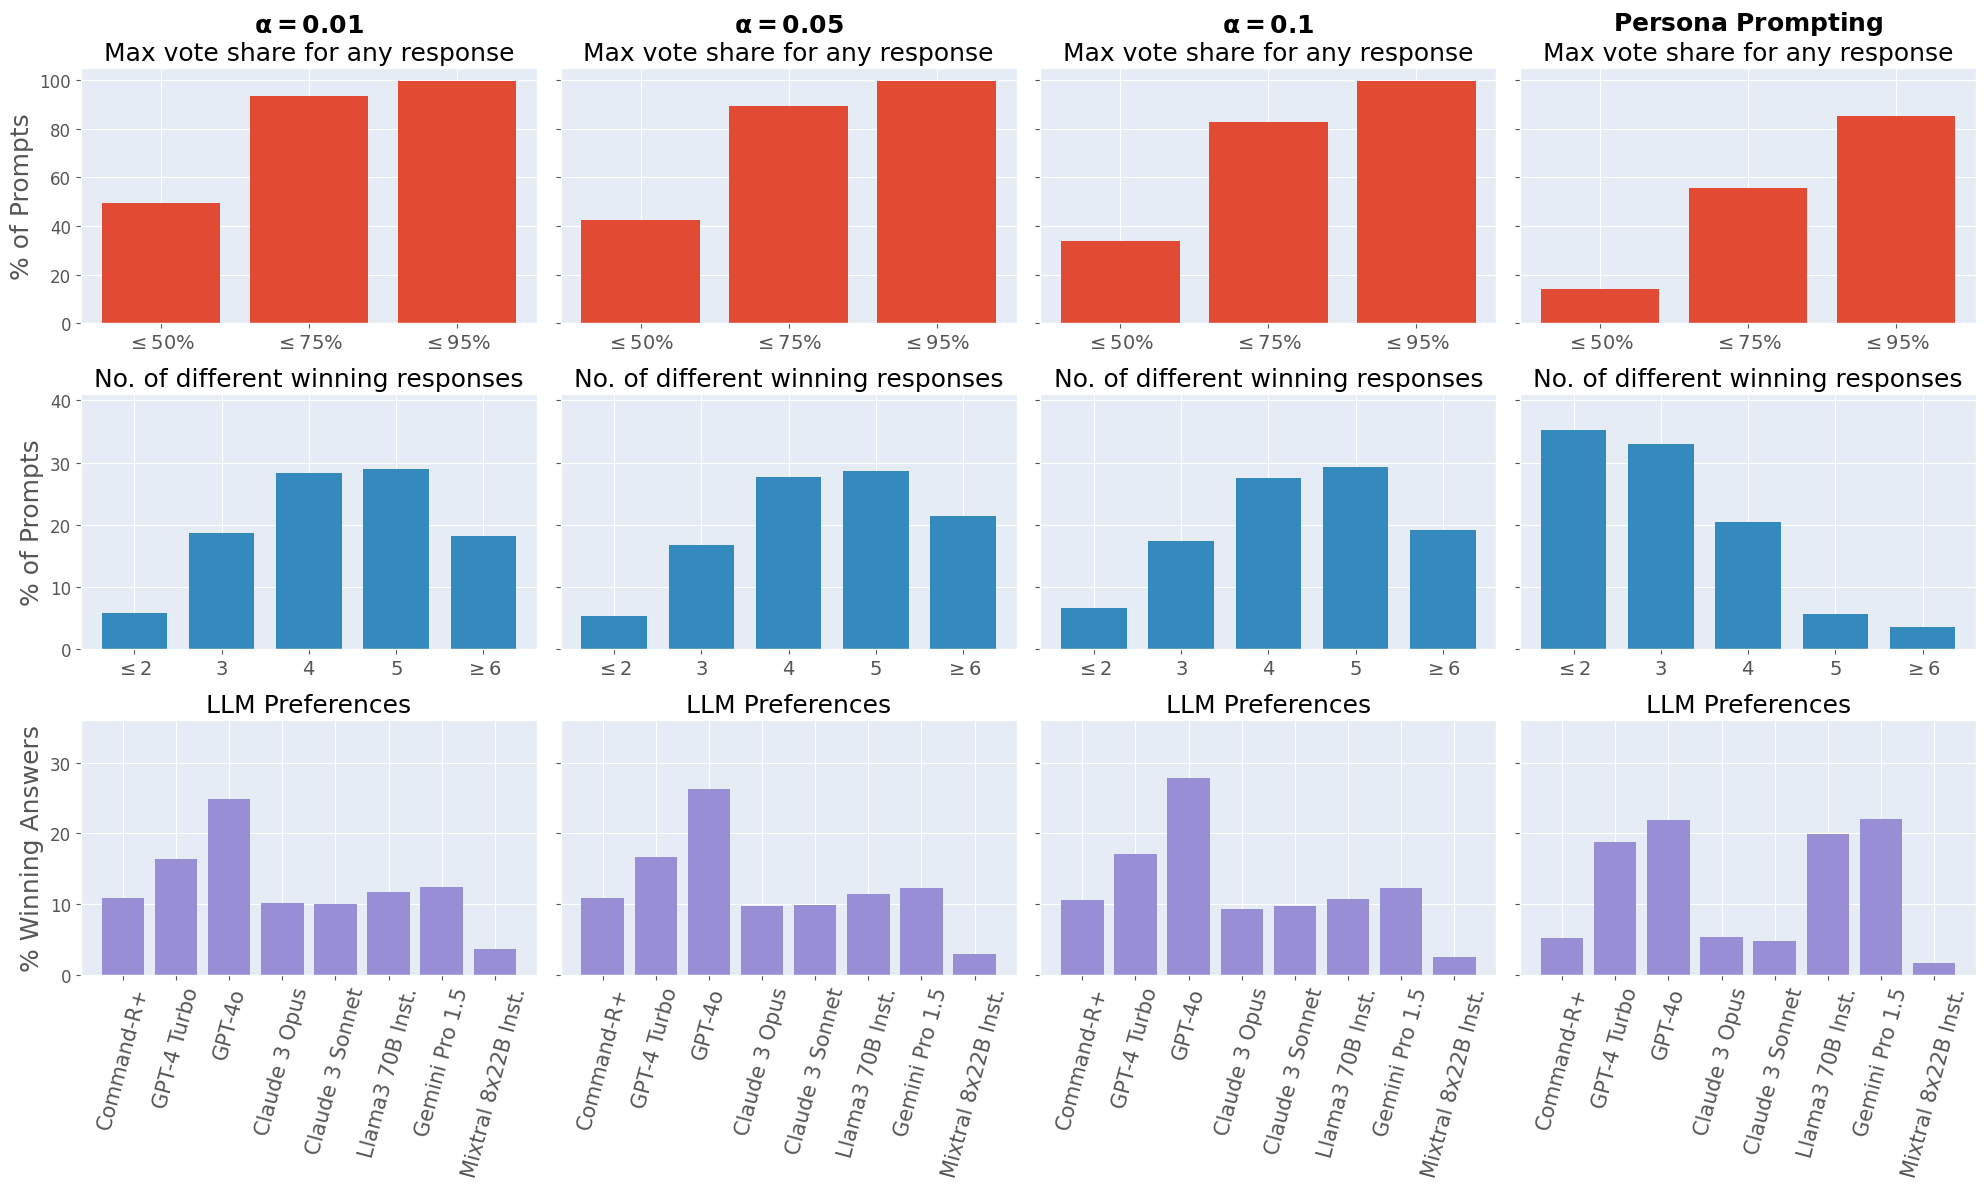
\includegraphics[width=\linewidth]{../figures/persona_prompting_comparison.png}
    \caption{Probing the heterogeneous preferences across \textsf{PersonalLLM} prompt/responses given different settings of $\alpha$, and comparing to a persona prompting baseline.  \textbf{Top}: For a population of simulated users, the percentage of each population's vote share given to the most common winning response for each prompt; higher values indicate more preference diversity. \textbf{Middle}: A histogram showing the number of responses that receive at least one vote from a simulated population for each prompt; diverse preferences cause higher concentration on the right side of each plot. \textbf{Bottom}: Average win rates across the population for the 8 LLMs in our dataset.}
    \label{fig:persona_diversity}
\end{figure}

\section{Analyzing PersonalLLM}\label{sec:persona_analysis}

Next, in order to validate our testbed, we explore the preferences exhibited by our simulated users over the \textsf{PersonalLLM} dataset.  

\subsection{Preference Diversity and Comparison to Persona Prompting}
% \hntodo{Enlarge figure titles, axis labels A LOT! Rule of thumb is whether it's clearly legible if printed on a letter sized paper. Figure 4 is especially challenging to read since the x-axis is different across rows. In the caption, it may be worth explicitly saying higher proportions on the left hand side implies greater diversity or something like this to help people skim the figure.}

First, we examine whether populations of personal preference models sampled via the method outlined in Section~\ref{sec:sim_users} do in fact display heterogeneous preferences over the prompt/response pair in our dataset.
In Figure~\ref{fig:persona_diversity} (left 3 columns), we provide experimental results for user bases of 1,000 \textsf{PersonalLLM} personal preference models sampled with parameters $\alpha=[0.01, 0.05, 0.1]$ and applied to the \textsf{PersonalLLM} test set to choose winning responses among the 8 included.
The top row displays the percentage of prompts in the dataset for which the most popular winning response according to the population receives no more than 50\%, 75\%, and 95\% of the population vote; higher values indicate more diversity in preferred responses.  
The middle row shows the percentage of prompts that have a given number of responses with at least one winning vote across the population; heterogeneous population preferences induce higher concentration on the right side of each plot.
On the bottom, we plot the overall win rates for each LLM across all users and prompts.

In the right column, we also offer results for a persona prompting baseline.  
Persona prompting \citep{castricato2024personareproducibletestbedpluralistic, chan2024scalingsyntheticdatacreation, jang2023personalizedsoupspersonalizedlarge} is an emerging method for evaluating methods for LLM personalization, wherein an LLM is prompted to decide which response would be preferred by a person of a particular race, gender, age, profession, or other demographic category.  
While one might argue that such evaluation is \textit{prima facie} discriminatory and reductive, and therefore not a desirable standard for algorithmic advancement, especially in sensitive areas, we are also interested in whether persona prompting meets the technical challenge of producing a simulation environment with a high degree of heterogeneity.
For our baseline, we prompt the sfairXC/FsfairX-LLaMA3-RM-v0.1 reward model \citep{dong2023raft} to score responses with respect to 500 personas randomly sampled from PersonaHub \citet{chan2024scalingsyntheticdatacreation}, a recent effort at building a database of personas that are representative of a pluralistic population.

Results are shown in Figure~\ref{fig:persona_diversity}.
For \textsf{PersonalLLM} personas, we can see that the top response receives a majority user vote for only about half of the prompts, while that figure is closer to 90\% for the persona prompting baseline.  
Also, for roughly 60\% of prompts, at least 5 different answers are chosen as the best by at least 1 under our set of personas; for LLM persona prompting, it is roughly 30\%.  
Finally, our ensembled preference models have a fairly diffuse set of preferences over the response-generating LLMs, while persona prompting strongly prefers a subset of 4 models.
With respect to changes across the left 3 columns, we can observe that as $\alpha$ increases, preferences become more uniform.  
However, if $\alpha$ is set too low, user preferences cluster very tightly around the base reward models; we observe this behavior for $\alpha=0.01$.

\begin{figure}[t]
    \centering 
    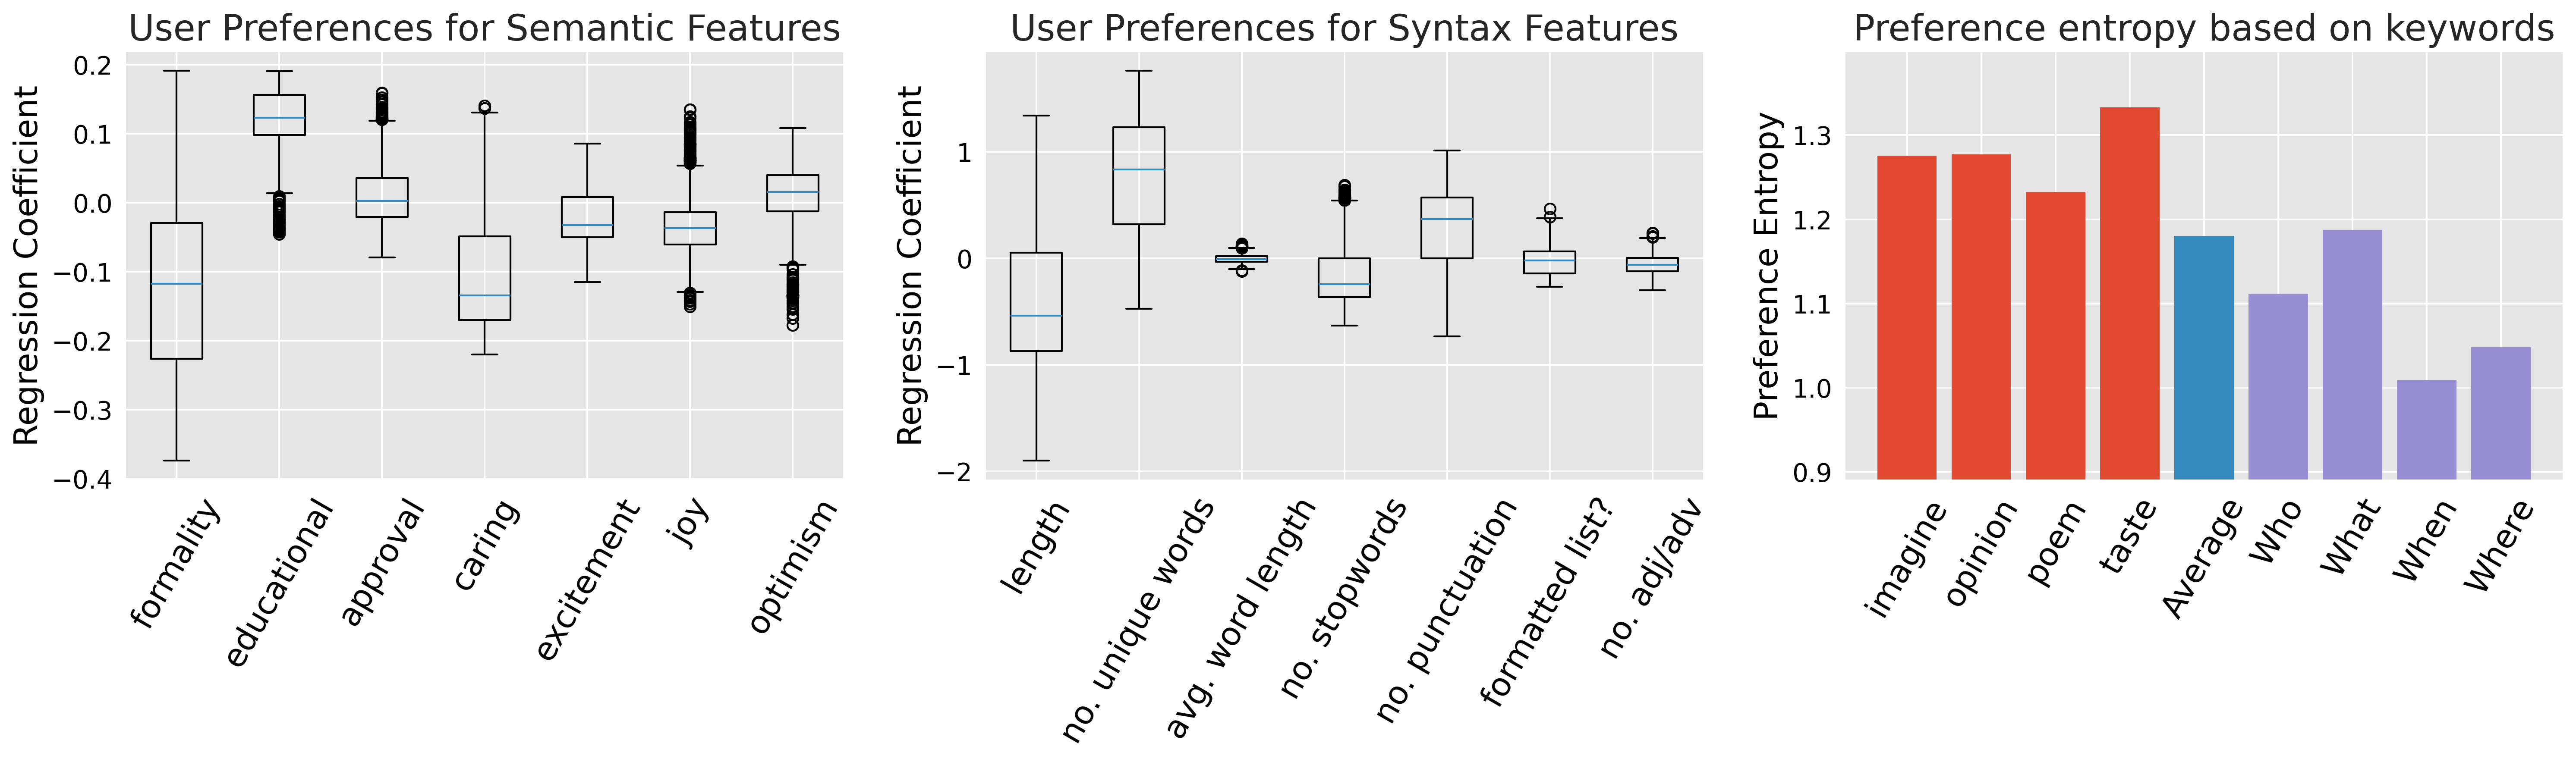
\includegraphics[width=\linewidth]{../figures/syn_sem_ent.png}
    \caption{Analysis of simulated user preferences with respect to prompt and response contents.
    \textbf{Left, middle:} For each user, we train a regression model to predict winning responses based on either semantic (left) or syntactic (middle) features.  For each feature, we show a box plot with the resultant regression coefficient across users.
    \textbf{Right:} We examine the entropy in population preferences based on keywords in prompts, comparing words we would expect to inspire heterogeneity (e.g., imagine, opinion, poem) to prompts beginning with who, when, and where, which should evoke more objective answers. 
    }
    \label{fig:sem_syn}
\end{figure}

\subsection{Effects of Semantics and Syntax}

% \hntodo{Enlarge figure titles, axis labels A LOT! Rule of thumb is whether it's clearly legible if printed on a letter sized paper}

We further analyze the effects of semantics and syntax on the preferences of a simulated user base (with $\alpha=0.05$ and 1,000 users).  We use regression analysis to understand how different features may drive the preferences of different users, including semantic response features such as the formality or educational value or the expressions of certain emotions (approval, caring, excitement, joy, optimism), as well as syntactic features like length and the use of different parts of speech and formatting.
For each user, we gather their most and least preferred responses for each of the test prompts, and create a binary prediction problem to predict whether a given response is a winning or losing response.
Responses are embedded using hand-crafted features (based on either syntax or semantics, which are studied separately), and a unique logistic regression model is trained \textit{for each user}.
Semantic features were captured using pretrained classifiers, while syntactic features were engineered using nltk \citep{bird-loper-2004-nltk}.  See Appendix \ref{app:user_details} for complete details.

In Figure~\ref{fig:sem_syn} (left and middle), for each feature we show a box plot with the resultant regression coefficient for that feature across users.  A positive coefficient suggests a feature associated with winning responses, while a negative coefficient suggests a feature's role in losing responses.  A tight box indicates homogeneous preferences, while a greater spread represents heterogeneity.
Here, we can see a reasonable mix of heterogeneity and homogeneity across user preferences for different features. 
Semantically, users tend to prefer responses with educational value and dislike highly formal responses, although the size of these preferences varies.
Encouragingly, syntactic preferences do not seem to be driven by uniform preferences for simple features like length or the presence of formatting such as bullets or lists.

In Figure~\ref{fig:sem_syn} (right), we compare the entropy in the population preferences over the responses to a given prompt based on keywords, comparing words we would expect to inspire heterogeneity (e.g., imagine, opinion, poem) to prompts beginning with who, when, and where, which evoke more objective answers.  We can see that the presence of these subjective cues leads to a more diverse set of preferences than those seeking simple entity or date responses.  Such diversity among the prompts creates a setting where an algorithm \textit{must not only learn how to personalize, but also when to personalize}.
% \hntodo{Consider moving much of the figure descriptions to the caption. Currently readers will need to read the subsection carefully to comprehend the plots. Most will start with the initial paragraph and then move to the figure to stare at them.}

\subsection{Comparison to Human Preferences}

% \hntodo{Perhaps give a couple of real examples from OpinionQA to ground our analysis.}
Finally, to understand how our synthetic personal preference models relate to human preferences over text responses, we surveyed a population of our simulated users on a set of questions with responses where a large and diverse set of humans have given their preferences in the past, the OpinionQA dataset
% , emulating the work of 
\citep{santurkar2023opinions}.
OpinionQA is an appropriate validation set for our personas given that its broad coverage of topics (e.g., science, economics, politics, romance, and many other topics) aligns with the open-domain nature of our prompt set.  See Table~\ref{tab:opinion_qa_examples} for example questions and answers.

\begin{table}[!ht]
    \centering
    \begin{tabular}{p{0.55\textwidth} p{0.4\textwidth}}
    \toprule
     Question & Answer\\
    \midrule
    How worried are you, if at all, about the possibility of using computer programs to make hiring decisions for society as a whole? & [Very worried, Somewhat worried, Not too worried, Not at all worried] \\
    \midrule
    Do you think men and women are basically similar or basically different when it comes to their hobbies and personal interests? & [Men and women are basically similar, Men and women are basically different] \\
    \bottomrule
    \end{tabular}
    \caption{Example questions and answers from the OpinionQA dataset.}
    \label{tab:opinion_qa_examples}

\end{table}

Following this previous work, we calculate the representativeness score of the opinion distribution given by our simulated preference models.
This score is based on the Wasserstein distance of the synthetic population preferences from that of real human populations for each question.
To have a high representativeness score, our simulated user population would have to display heterogeneous preferences over question/response sets where humans do so, and produce homogeneous (and matching) preferences in cases where humans do the same. 

Our population of simulated users produces a representativeness score of 0.839 with respect to the overall population of the US, higher than any LLM in the original study and near as representative of the overall population as some real, large demographic groups.  
Further, in Table~\ref{tab:opinion_qa} we can see that our simulated users produce opinions that better represent a wide range of important (and sometimes protected) groups according to demographic attributes such as race, political leaning, religion, marital status, and more.  
In fact, this is the case for 59 of 60 demographic groups in their study (see Appendix Table~\ref{tab:opinion_qa_full}).

\begin{table}[!ht]
    \centering
    \begin{tabular}{lccccc}
    \toprule
     & \multicolumn{2}{c}{AI21 Labs} & \multicolumn{2}{c}{OpenAI} & \textsf{PersonalLLM} \\
    Demographic & j1-jumbo & j1-grande-v2 & ada & text-davinci-003 & \textbf{Ours} \\
    \midrule
    Asian & 0.814 & 0.806 & 0.819 & 0.708 & \textbf{0.839} \\
    Black & 0.820 & 0.812 & 0.823 & 0.702 & \textbf{0.833} \\
    Hispanic & 0.820 & 0.810 & 0.824 & 0.706 & \textbf{0.839} \\
    White & 0.807 & 0.794 & 0.817 & 0.699 & \textbf{0.832} \\
    Conservative & 0.796 & 0.780 & 0.810 & 0.684 & \textbf{0.817} \\
    Liberal & 0.792 & 0.788 & 0.799 & 0.721 & \textbf{0.833} \\
    Democrat & 0.800 & 0.795 & 0.804 & 0.719 & \textbf{0.834} \\
    Republican & 0.791 & 0.776 & 0.805 & 0.680 & \textbf{0.812} \\
    Muslim & 0.794 & 0.788 & 0.792 & 0.697 & \textbf{0.816} \\
    Roman Catholic & 0.816 & 0.806 & 0.823 & 0.702 & \textbf{0.835} \\
    Less than \$30,000 & 0.828 & 0.813 & 0.833 & 0.693 & \textbf{0.838} \\
    \$100,000 or more & 0.797 & 0.790 & 0.807 & 0.708 & \textbf{0.831} \\
    18-29 & 0.818 & 0.808 & 0.828 & 0.700 & \textbf{0.840} \\
    65+ & 0.792 & 0.779 & 0.800 & 0.699 & \textbf{0.818} \\
    Divorced & 0.809 & 0.796 & 0.817 & 0.696 & \textbf{0.830} \\
    Married & 0.810 & 0.799 & 0.819 & 0.699 & \textbf{0.832} \\
    \bottomrule
    \end{tabular}
    \caption{Representativeness scores in relation to real human opinions from important demographic groups for different LLMs, as well as our \textsf{PersonalLLM} population.}
    \label{tab:opinion_qa}
\end{table}

\subsection{Summary of Analysis}

Taken together, these results show that our simulated user reward models: 1) produce heterogeneous preferences over our dataset of prompts and responses, considerably more so than persona prompting an LLM, 2) display reasonable and diverse preferences with respect to syntactic and semantic content of prompts, and 3) simulate a user base that better represents diverse human opinions than many popular LLMs, without resorting to explicit stereotyping.
% \hntodo{Claiming better representation of real human opinions may be untenable. One option is to focus on diversity and heterogeneity rather than realism.}



\section{Personalization Experiments}\label{sec:experiments}

A central challenge in personalization is the perpetual lack of data, as most users will provide sparse feedback, far
% fewer 
less
than necessary to effectively adapt an LLM.
Two first-order problems emerge from such an environment: 1) how to best leverage small amounts of user-specific data for personalized adaptation and 2) how to lookup similar users based on language feedback.
In order to illustrate how researchers might approach these problems, we perform experiments in two modal settings for LLM personalization research.
First, we explore a scenario where we have access to a short but relevant interaction history for the user, and we aim to efficiently leverage that interaction history through ICL.  
Then, we explore a more complex setting that fully leverages the advantages of \textsf{PersonalLLM}, where the current user possibly has no relevant interaction history, and we must instead retrieve relevant interactions from similar users in a database.
Overall, our results validate the solid empirical foundations of \textsf{PersonalLLM} while highlighting salient algorithmic questions and the fact that there is much room for improvement in terms of personalization performance.

All experiments simulate a chatbot using in-context learning to personalize responses for a test set of new users.
Our test set simulates 1,000 personal preference models (or ``users'') drawn with $\alpha=0.05$ (as in the analysis in Section~\ref{sec:persona_analysis}), and each user is associated with one test prompt from the \textsf{PersonalLLM} test split.
For a new user with an associated test prompt, the goal is to use ICL to produce a response to maximize the reward (and win rate vs. GPT4o) given by the user's personal preference model (i.e., weighted ensemble of reward models).
Our underlying chatbot is Llama3-8B-Instruct, and all embeddings are extracted using dunzhang/stella\_en\_400M\_v5, which is the top-ranking model on the MTEB \citep{muennighoff2023mtebmassivetextembedding} leaderboard below 500M parameters.
Further details for each individual experiment are given below and in Appendix \ref{app:exp_details}.

\subsection{Personalized In-Context Learning}

While ICL for broad alignment has been studied to some extent \citep{lin2023unlockingspellbasellms}, the problem may be different when the underlying preference model is idiosyncratic and may cut against pretraining and RLHF dataset biases.
In our initial set of experiments, we focus on a setting wherein we have a small set of useful data for the sake of personalizing the response to a given query, i.e., feedback gathered from the same user on similar prompts.  
By doing so, we can study key questions related to personalized inference with ICL, for example which response(s) should be included and the importance of correct labels.  
Though these questions have been studied with respect to more general NLP tasks \citep{min2022rethinkingroledemonstrationsmakes, yoo2022groundtruthlabelsmatterdeeper, pan2023incontextlearninglearnsincontext}, it is unlikely that these findings can be extrapolated to the unique personalization task, and thus more work is needed in this area.
A solid foundation of ICL techniques for personalization can then form the basis for more complex systems involving, e.g., looking up similar users.

% \TZ{Give analogy to related work in non-personalized ICL}
% \hntodo{I suggest beginning with why this experiment is interesting and has implications for future methodological development. IMO, retrieval for personalization is a wide-open direction and we're showing that the simplest innovations in retrieval schemes can have impacts on overall personalization performance.}
% \TZ{This is not really about retrieval/RAG?  It's more about how to do ICL, given a fixed set of in-context examples.}
% \hntodo{I think the realistic analogue of this setting will be a platform having a wealth of interactions with each user, yet needing to understand which one is most relevant for the current prompt. I understand this is not something we study atm, but it'll be good to depict a broader vision.}


\subsubsection{Experiment Details}

For each of our 1,000 test users, each with their own test prompt, we build a short but relevant interaction history by retrieving 5 other prompts based on embedding similarity. We build a winning/losing response pair for each prompt based on each user's most and least preferred answers from the 8 models in our dataset.  In order to establish baseline results on key questions in personalization, we include several baselines for how these interaction samples are leveraged in-context during inference: 
\begin{itemize}
    \item \textbf{Winning and Losing:} Both the winning and losing responses are included.
    \item \textbf{Winning only:} Only the winning response is included.
    \item \textbf{Losing only:} Only the losing response is included.
    \item \textbf{Losing only (Mislabeled):} Only the losing response is included, and it is mislabeled as a winning response.
\end{itemize}
Inference is performed using 1, 3, and 5 such examples (see Appendix \ref{app:exp_details} for exact templates), and evaluated by scoring with each user's (weighted-ensembled) preference model.  We also compare to a zero-shot baseline, with no personalization.

\subsubsection{Results}

Results are shown in Figure~\ref{fig:exp_results}, left column.  
We can see that the best performance comes from ICL with only winning examples. 
This underlines the outstanding issue of training LLMs to not only mimic winning responses in-context, but also leverage the contrast between winning and losing responses, especially when the differences may not described in the model's training data.
Any amount of examples, even incorrectly labeled, are helpful relative to zero-shot; this may be unsurprising, as all 8 models in our dataset are stronger than our 8B parameter chat model.
An interesting result lies in the comparison between Losing Only and Losing Only (Mislabeled).  
While the mislabeled examples may help performance versus a zero-shot baseline (once again because they are from a stronger underlying LLM), Llama-8B-Instruct gains more from having these relatively strong losing responses labeled as losing.
Overall, our findings reflect that a model trained for broad alignment does have some of the necessary capabilities to do idiosyncratic personalization using only in-context examples, but that much work is left in order to fully leverage this language feedback.
% \hntodo{There is a rich literature on ICL retrieval. Probably worth citing a few to attribute credit.}

\begin{figure}[!ht]
    \centering
    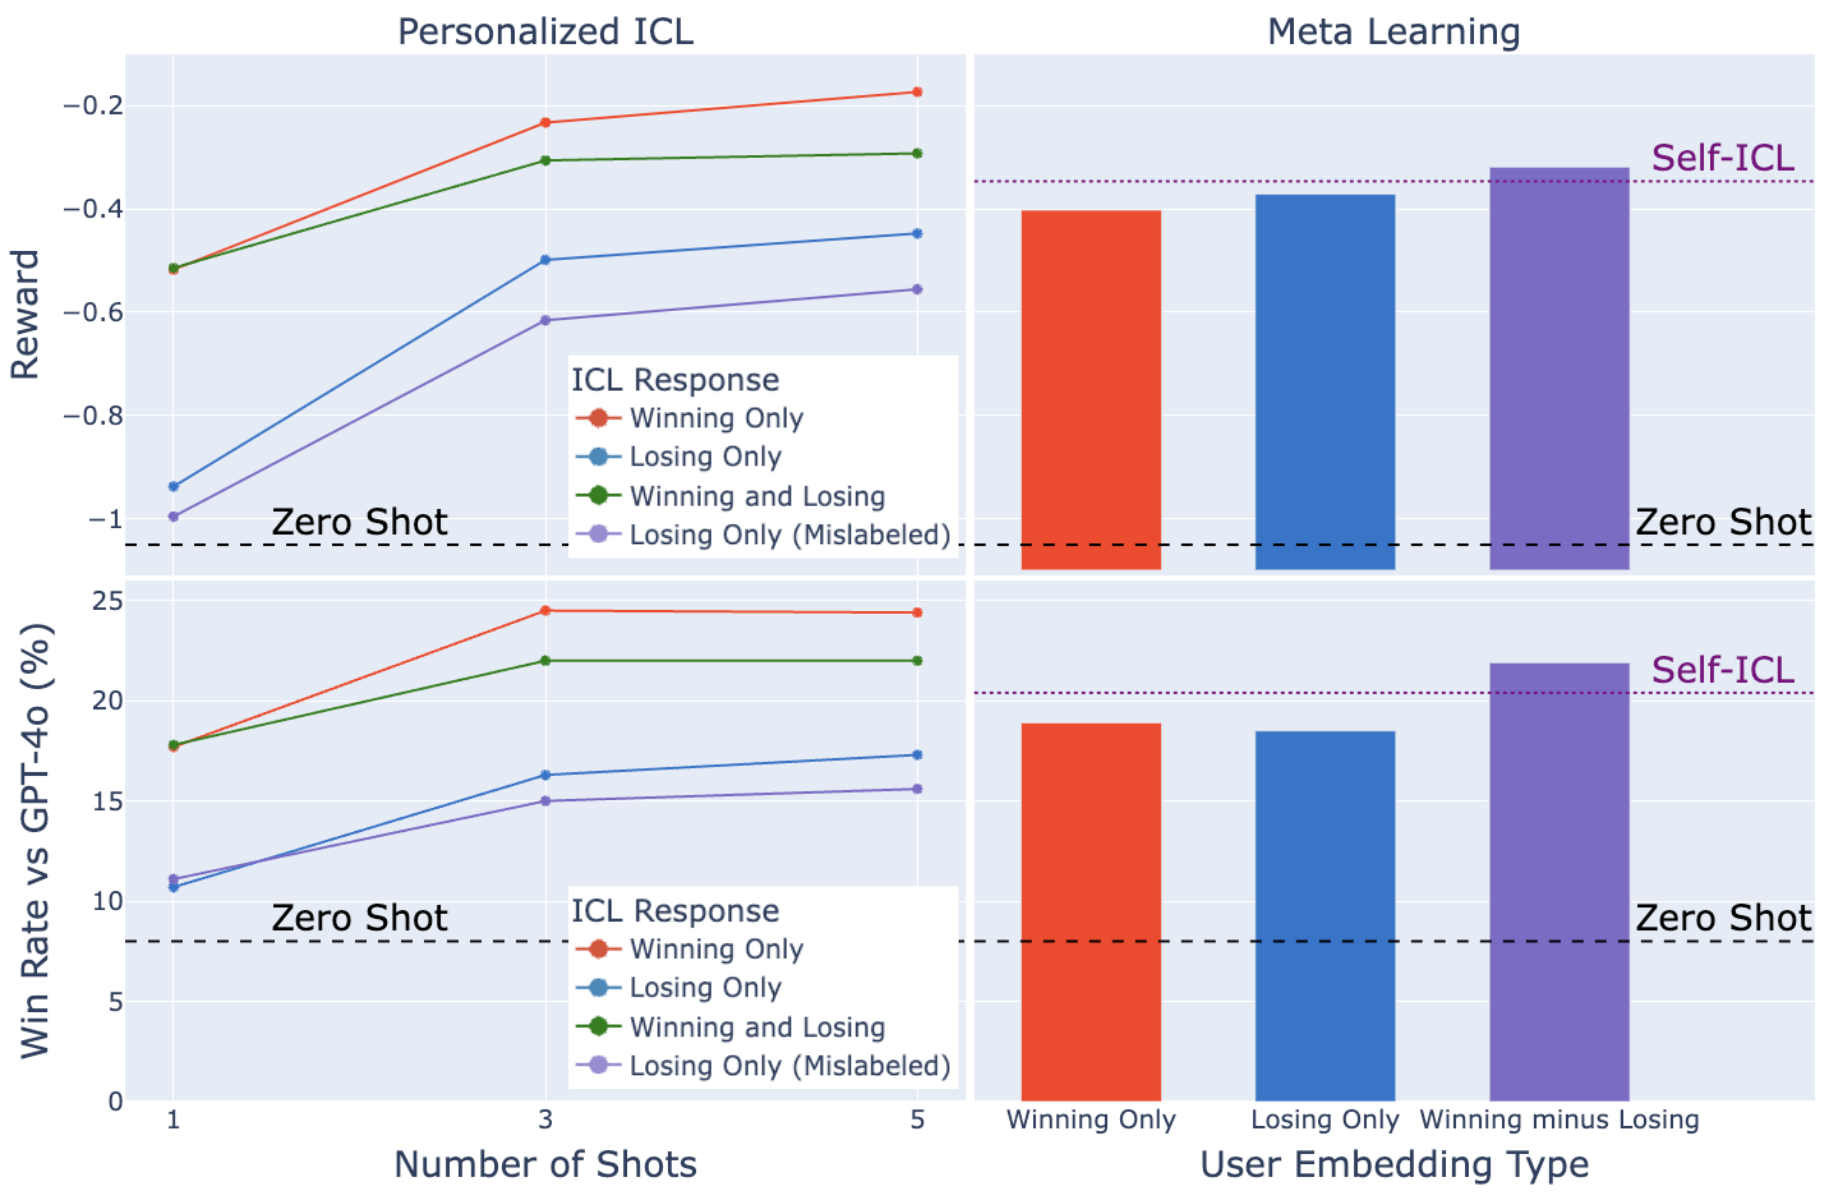
\includegraphics[width=\textwidth]{../figures/fig6sharp.png}
    \caption{Results across different personalization algorithms. 
    \textbf{(Left)} Test users are accompanied by a relevant interaction history with pairwise preference feedback, and we explore the LLM's ability to exploit this information in context. 
    \textbf{(Right)} Test users have interaction histories that are not relevant to their test prompt, and we probe methods for embedding users based on language feedback to retrieve useful examples from simular users for ICL.}
    \label{fig:exp_results}
\end{figure}


\subsection{Learning Across Users}

Having established some empirical foundations for in-context personalization with \textsf{PersonalLLM}, we next highlight a particularly significant challenge prevalent in practice that has been under-explored in the LLM community: the cold-start problem. 
When a new user with limited prior interaction data arrives, or a user inquires about a new topic, prior user interactions alone cannot inform a satisfactory response.
We model this challenge as a meta-learning problem, where the goal is to utilize a rich reservoir of prior interactions with a diverse set of users. 
We are motivated by real-world scenarios where we have access to a proprietary database containing extensive interaction histories from previous users. 
When a new user arrives, our goal is to utilize this rich, heterogeneous dataset to provide the best possible response to the new user's query despite having only limited initial interactions with them that may not be relevant to the current query. 
This setting resembles typical recommendation systems, but "actions" are now defined over the space of natural language outputs instead of a fixed set of items.
See Figure~\ref{fig:metalearn} for further illustration.

Our experiment explores the open question of how best to embed (e.g., represent with some vector) users based on small amounts of natural language feedback.  
With effective algorithms to lookup similar users, more relevant interactions may be leveraged to improve a response to a new user query.
While a rich literature exists on information retrieval (i.e., RAG) for typical NLP benchmark tasks like question answering and fact checking \citep{lewis2021retrievalaugmentedgenerationknowledgeintensivenlp, gao2024retrievalaugmentedgenerationlargelanguage}, the distinctive nature of the personalization task necessitates new algorithms.

\subsubsection{Experiment Details}

For each of our 1,000 test users, we build a short but, in contrast to our first experiment, \textit{possibly irrelevant} interaction history by retrieving 5 random prompts.  Winning/losing response pairs (i.e., preference feedback) are selected as before.  In order to supplement these interaction histories, we sample a historical database of 10,000 users (also with $\alpha=0.05$), each with a set of 50 prompt, winning response, losing response triplets from the train set, where the prompts are selected randomly and the winning and losing responses are selected as the historical user's highest and lowest scoring among the 8.

We compare 3 methods for embedding users for lookup:
\begin{itemize}
    \item \textbf{Winning minus Losing:} Average direction in embedding space between winning and losing responses for each prompt.
    \item \textbf{Winning only:} Average direction in embedding space for winning responses. 
    \item \textbf{Losing only:} Average direction in embedding space for losing responses.
\end{itemize}

For each test user, we build a set of candidate prompt/feedback data by retrieving the 20 most similar historical users based on cosine similarity of their embeddings, and then of the pool created by those users' interaction histories, retrieving 3 examples for in-context learning based on prompt embedding similarity to the user's test prompt.  We compare to a \textbf{Self-ICL} baseline, where the test user's possibly irrelevant prompt/feedback history is used for ICL.  Evaluation is done as before.

\subsubsection{Results}

Our results are shown in Figure~\ref{fig:exp_results}.  
We find that using the strongest user embedding method, which most fully exploits the available pairwise preference feedback, meta-learning can beat the self-ICL baseline.
This positive result for meta-learning highlights the opportunity created by leveraging historical user data, and the feasibility of embedding users based on a small amount of language feedback.
However, the gain from our relatively naive method is small, illustrating the need for methodological innovation in building such systems.

\section{Related Work}


\paragraph{Preference Datasets}
Recent developments in large language models (LLMs) emphasize the importance of \emph{aligning} LLMs based on \emph{preference feedback} rather than merely pre-training on large corpora of language in a self-supervised manner. 
Consequently, there has been a surge in the creation of open-source datasets \citep{bai2022training, nakano2022webgpt, köpf2023openassistant, dubois2024alpacafarm, lambert2024rewardbench} designed to support research on alignment methodologies. A significant limitation in the existing datasets is that they mainly enable fine-tuning to a single high-level notion of alignment that is uniform across the population, such as instruction-following in RLHF~\citep{ouyang2022training} and helpfulness and harmlessness \citep{bai2022training}. 

\paragraph{Personalization}

Personalization has been extensively researched across different fields, with previous datasets primarily focusing on applications such as search engines and recommender systems \citep{davidson2010youtube, das2007google, Xu_2022, F_rber_2020}. 
Where personalization has been studied in NLP, it has traditionally been focused on learning to mimic a user's style, for example in writing headlines \citep{ao-etal-2021-pens}, crafting social media posts \citep{mazare-etal-2018-training}, or emulating historical text with simple dialogue models \citep{wu-etal-2021-personalized}.

Recently, given the success of population-level alignment, researchers have begun to develop testbeds and methodology wherein the goal is to achieve a more granular level of personalized alignment for LLMs \citep{castricato2024personareproducibletestbedpluralistic, jang2023personalizedsoupspersonalizedlarge, kirk2024prismalignmentprojectparticipatory, li2024personalizedlanguagemodelingpersonalized}.
Much of this work has focused on alignment for real or synthetic personas based on high-level attributes like race or occupation \citep{castricato2024personareproducibletestbedpluralistic, chan2024scalingsyntheticdatacreation}, or high-level notions of alignment with respect to response qualities like length, technicality, and style.  
For example, \citet{jang2023personalizedsoupspersonalizedlarge} decomposes personal preferences along a handful of easily observable dimensions and performs personalized generation by merging models trained with different preference data based on these dimensions.
Evaluation is often done by prompting GPT4 to select the preferred response based on preferences stated in its prompt \citep{jang2023personalizedsoupspersonalizedlarge, castricato2024personareproducibletestbedpluralistic}.  
In an effort to highlight the need for broad participation and representation in LLM alignment, the PRISM dataset collects user-profiles and personalized preference feedback from over 1,000 diverse human participants \citep{kirk2024prismalignmentprojectparticipatory}.



\vspace{-5pt}
\section{Discussion}\label{sec:discussion}
\vspace{-5pt}

We present \textsf{PersonalLLM}, a dataset and benchmark meant to spur the development of algorithms for LLM personalization, a critical and under-explored area with significant potential for enhancing interaction quality.   We discuss the potential of the empirical foundation we develop and highlight potential risks and limitations.


\paragraph{Meta-Learning for Personalization}
We hope to encourage more work in the meta-learning setting, as exemplified by our experiments. This setting mirrors many real-world use cases where an organization has a large proprietary dataset from historical users but a very limited interaction history with this particular user. 
Prior work on cold-start problems has focused on the task of recommending discrete content items from a media (or other) library. 
Extending and developing these techniques for LLMs is an exciting direction for future research. 

\paragraph{Risks and Limitations} 
We must consider the risks and limitations associated both with the release of our original benchmark dataset, as well as the larger goal of LLM personalization.

With respect to \textsf{PersonalLLM}, we note all prompts and responses have not been manually inspected for quality or safety by a human, although prompts are sourced from existing, reputable datasets, and responses are generated from state-of-the-art language models that have (presumably in the case of black box models) undergone safety alignment.
Our benchmark is also limited with respect to the realism of the personas created by weighting reward models.

On a broader note, the goal of LLM personalization brings particular risks.
One common concern is the creation of filter bubbles, where the model's outputs become increasingly tailored to the user's past existing preferences, potentially reinforcing political beliefs and biases, isolating the user from opposing viewpoints, and narrowing the diversity of information presented.
Another potential issue is stereotyping, where the model may perpetuate or even amplify biases based on the user's demographic information or behavior patterns.
Feedback loops may also emerge, where the model behavior affects human behavior and vice versa, leading to negative personal and unknown societal consequences.
Personification risks arise, as over time the user may develop a pseudo-personal relationship with the user, potentially fostering over-reliance on the LLM for advice or companionship. Finally, 
if used by malicious actors, personalized
LLMs can be employed to manipulate and extort
individuals by exploiting personal levers.
Given these and many other predictable (and unpredictable) potential risks, it is important that any efforts at LLM personalization are accompanied by research in robust transparency mechanisms and safeguards for personalization algorithms. Developing an empirical foundation for such efforts is another promising avenue for future work.

\paragraph{Future Directions} Given that LLMs have only recently reached a level of capabilities meriting their widespread adoption for industrial and personal use, the study of LLM personalization is necessarily in its earliest stages of development.  
It follows that there are many important and exciting avenues for future research, with respect to datasets, methodology, fairness, safety, and other aspects of responsible and reliable machine learning deployment.  
Since \textsf{PersonalLLM} is the first dataset to enable the study of complex personalized preferences expressed over many high-quality responses (to our knowledge) by a large, diverse user base, the benchmark can be extended in many ways. 
For example, one might imagine a distribution shift scenario, where over time, personal preferences shift, and the personalization algorithm must balance stability and plasticity.  
Also, we hope that our testbed drives the development of even more realistic personalization datasets and evaluation methods that more closely mirror the online and non-i.i.d.~nature of the conversational setting and more closely capture the true nuance and diversity of human personal preferences.  Finally, continued work in personalization algorithms must be accompanied by a proportional amount of work in personalization safety, fairness, and reliability.  Future research may consider different aspects of the deployment pipeline (e.g., model architecture, data collection) and interaction model (e.g., UI/UX) with these concerns in mind.





\newpage
\bibliographystyle{plainnat}
\bibliography{../cite.bib}

\newpage
\begin{appendix}

    

\section{Dataset Information}\label{app:add_data_det}

This section serves as documentation for our dataset, with its organization based on the notion of datasheets \citep{gebru2021datasheets}.

Our dataset is available at \url{https://huggingface.co/datasets/namkoong-lab/PersonalLLM}.

The code used to collect, process, and score our dataset (and run our experiments) is available at \url{https://github.com/namkoong-lab/PersonalLLM}.

The evaluation dataset that we used to produce our experiments in Section 4 is available at \url{https://huggingface.co/datasets/namkoong-lab/PersonalLLM_Eval}.

The interaction database dataset that we constructed from PersonalLLM is available at \url{https://huggingface.co/datasets/namkoong-lab/PersonalLLM_InteractionDatabase}.

\subsection{Composition}

\subsubsection{Prompts}

In order to create a set of prompts and responses over which humans (and reward models) will display diverse preferences, our first focus was the collection of \textit{open-ended} prompts.
As a source of these open-ended prompts, we collected data from \textbf{Anthropic Helpful-online}, \textbf{Anthropic Helpful-base}, \textbf{Nvidia Helpsteer}, and \textbf{RewardBench}.
From this set, prompts were filtered to those with a length of 2400 characters or fewer as most reward models are limited to 4096 context length. We randomly drew 10,402 prompts from the filtered subset.  The resulting distribution of prompts from different sources is shown in Table~\ref{tab:prompt_sources}.

\begin{table}[!ht]
    \centering
    \begin{tabular}{cc}
        \toprule
        Source & Count \\
        \midrule
        hh-rlhf-helpful-base & 4797 \\
        hh-rlhf-helpful-online & 3320 \\
        HelpSteer & 1290 \\
        alpacaeval-hard & 285 \\
        alpacaeval-easy & 259 \\
        alpacaeval-length & 219 \\
        xstest-should-respond & 65 \\
        llmbar-adver-neighbor & 43 \\
        llmbar-adver-GPTInst & 34 \\
        llmbar-natural & 27 \\
        llmbar-adver-manual & 19 \\
        llmbar-adver-GPTOut & 15 \\
        mt-bench-med & 14 \\
        mt-bench-hard & 10 \\
        mt-bench-easy & 5 \\
        \bottomrule
    \end{tabular}
    \caption{Sources of the 10,402 prompts composing our train and test sets.}
    \label{tab:prompt_sources}
\end{table}

\subsubsection{Responses}

Next, we aimed to collect many high-quality responses for each prompt. 
We generated eight responses for each of the 10,402 prompts using a selection of the top models from ChatArena and other important benchmarks: \textbf{GPT-4o}, \textbf{Claude 3 Opus}, \textbf{Gemini-Pro-1.5}, \textbf{Command-R-Plus}, \textbf{GPT-4-Turbo}, \textbf{Claude 3 Sonnet}, \textbf{Llama3-70B-Instruct}, and \textbf{Mixtral 8x22B}. We split the resulting dataset into training and test sets in a roughly 9:1 ratio, with a final count of 9,402 training examples and 1,000 test examples.

\subsubsection{Reward Models}

Finally, in order to enable the simulation of many diverse preference models, we select 10 reward models from Reward Bench, built on top of popular base models such as Llama3, Mistral, and Gemma.  Their model names on Huggingface are:  

\begin{itemize}
    \item hendrydong/Mistral-RM-for-RAFT-GSHF-v0 
    \item OpenAssistant/oasst-rm-2-pythia-6.9b-epoch-1
    \item OpenAssistant/oasst-rm-2.1-pythia-1.4b-epoch-2.5
    \item OpenAssistant/reward-model-deberta-v3-large-v2
    \item PKU-Alignment/beaver-7b-v1.0-cost 
    \item Ray2333/reward-model-Mistral-7B-instruct-Unified-Feedback
    \item sfairXC/FsfairX-LLaMA3-RM-v0.1
    \item weqweasdas/RM-Gemma-2B 
    \item weqweasdas/RM-Gemma-7B 
    \item weqweasdas/RM-Mistral-7B 
\end{itemize}

We evaluate each (prompt, response) pair in the train and test set with each model so that for any personality created by their ensembling, each (prompt, response) pair in the dataset can be scored via a simple weighting.

\subsubsection{Data Records}

Each record in our resulting dataset is of the form
$$ (x,s,y_1,r_1^{(1)},...,r_1^{(k)},...,y_l,r_l^{(1)},...,r_l^{(k)}) $$
where $x$ is an input prompt, $s$ gives the source dataset for the prompt, $y_i$ is a response generated by the LLM indexed by $i$ among our set of $k=8$, and $r_i^{(j)}$ is the reward score for prompt/response pair $(x, y_i)$ by the reward model indexed by $j$ among a set of $l=10$ reward models in total.


\subsection{Collection Process}

Our prompts were collected by downloading and filtering the open source datasets mentioned previously.  Responses were generated using OpenRouter with a temperature of 1.0 and a maximum token length of 512.

\subsection{Preprocessing/cleaning/labeling}

All prompts are taken in their exact form from existing open source datasets, filtered by length according to Appendix A.1.1.  LLM responses are not filtered, edited, or cleaned in any way, either for storage or reward scoring.  

As a limitation, we note that all prompts and responses have not been manually inspected for quality or safety by a human, although prompts are sourced from existing, reputable datasets, and responses are generated from state-of-the-art language models that have (presumably in the case of black box models) undergone safety alignment.  Further, the personas that can be created via ensembling our reward models have not been tested for bias or alignment with a particular subgroup of the population.

We also note that there is a known issue with many reward models, such that they may produce different scores under different conditions, in particular when the batch size changes \footnote{https://github.com/allenai/reward-bench/issues/137}.  Our reward scores are produced with a batch size of 1, and is tested for reproducibility and determinism.

\subsection{Uses}

Our goal in creating the open-source PersonalLLM dataset is to facilitate work on methods to personalize the output of an LLM to the individual tastes of the many diverse users of an application.
In our initial paper, we have provided experiments where meta-learning and in-context learning (ICL) are used to leverage an existing user base with interaction histories to improve outcomes for new users.
We imagine further work in this direction, as well as potential work on more efficient ways to harness the power of fine-tuning for personalization. Also, in domains like medicine, where privacy is paramount, it may not be possible to include queries from other users in context.  Thus, work on privacy-ensuring meta-learning personalization algorithms is needed. 

It must be acknowledged that the goal of LLM personalization brings particular risks, including filter bubbles, stereotyping, feedback loops, personification, and manipulation.
Given these and many other predictable (and unpredictable) potential risks, it is important that any efforts at LLM personalization are accompanied by research in robust transparency mechanisms and safeguards for personalization algorithms.

\subsection{Distribution}

\subsubsection{Hosting}

PersonalLLM is available for download on huggingface at \url{https://huggingface.co/datasets/namkoong-lab/PersonalLLM}.

\subsubsection{License}

We release this dataset under a CC BY-NC 4.0 License, which prohibits commercial use and requires attribution.

\subsection{Maintenance}

The authors plan to maintain the dataset.  If any instances of dangerous, private, or otherwise undesirable material are found, the corresponding row in the dataset will be deleted.

Correspondence, including requests for data removal, can be sent to \url{andrew.siah@columbia.edu} and \url{tpz2105@columbia.edu}.


\section{Simulated User Analysis}\label{app:users}

\subsection{Additional Details}\label{app:user_details}

All semantic features are scored using pre-trained models from Huggingface.

\begin{itemize}
    \item Formality is scored using: s-nlp/roberta-base-formality-ranker
    \item Educational value is scored using: HuggingFaceFW/fineweb-edu-classifier
    \item Emotions are scored using: SamLowe/roberta-base-go\_emotions
\end{itemize}

Below is a list of our syntatic features:
\begin{itemize}
    \item Count of tokens
    \item Count of unique words
    \item Average word length
    \item Count of stopwords
    \item Count of punctuation
    \item Count of list items (bullets or numbered)
    \item Count of adjectives and Adverbs
\end{itemize}
The python package nltk \citep{bird-loper-2004-nltk} is used to tokenize, extract stopwords, and tag parts of speech, where necessary.

Our linear regression models are built using sklearn \citep{scikit-learn}, with default parameter settings.

\subsection{Additional Results}\label{app:user_results}

Tables~\ref{tab:opinion_qa_full} and \ref{tab:opinion_qa_full_2} show representativeness scores for our PersonalLLM users as well as a selection of LLMs across all 60 demographic groups in the original OpinionQA \citep{santurkar2023opinions} study.

\begin{table}[!ht]
    \centering
    \begin{tabular}{lccccc}
    \toprule
     & \multicolumn{2}{c}{AI21 Labs} & \multicolumn{2}{c}{OpenAI} & \textsf{PersonalLLM} \\
    Demographic & j1-jumbo & j1-grande-v2 & ada & text-davinci-003 & \textbf{Ours} \\
    \midrule
Northeast & 0.811 & 0.802 & 0.819 & 0.704 & 0.838 \\
Midwest & 0.810 & 0.797 & 0.820 & 0.701 & 0.833 \\
South & 0.818 & 0.805 & 0.827 & 0.696 & 0.835 \\
West & 0.813 & 0.802 & 0.821 & 0.704 & 0.839 \\
18-29 & 0.818 & 0.808 & 0.828 & 0.700 & 0.840 \\
30-49 & 0.814 & 0.804 & 0.823 & 0.702 & 0.837 \\
50-64 & 0.809 & 0.797 & 0.818 & 0.696 & 0.830 \\
65+ & 0.792 & 0.779 & 0.800 & 0.699 & 0.818 \\
Male & 0.814 & 0.802 & 0.826 & 0.697 & 0.837 \\
Female & 0.810 & 0.800 & 0.816 & 0.702 & 0.833 \\
Less than high school & 0.828 & 0.812 & 0.835 & 0.685 & 0.832 \\
High school graduate & 0.816 & 0.799 & 0.826 & 0.691 & 0.832 \\
Some college, no degree & 0.814 & 0.804 & 0.823 & 0.701 & 0.836 \\
Associate's degree & 0.811 & 0.800 & 0.821 & 0.700 & 0.834 \\
College graduate & 0.802 & 0.794 & 0.810 & 0.710 & 0.833 \\
Postgraduate & 0.794 & 0.789 & 0.800 & 0.717 & 0.831 \\
Citizen - Yes & 0.814 & 0.802 & 0.823 & 0.700 & 0.836 \\
Citizen - No & 0.816 & 0.812 & 0.818 & 0.706 & 0.833 \\
Married & 0.810 & 0.799 & 0.819 & 0.699 & 0.832 \\
Divorced & 0.809 & 0.796 & 0.817 & 0.696 & 0.830 \\
Separated & 0.814 & 0.801 & 0.818 & 0.694 & 0.830 \\
Widowed & 0.800 & 0.785 & 0.807 & 0.694 & 0.819 \\
Never been married & 0.819 & 0.808 & 0.828 & 0.700 & 0.841 \\
Protestant & 0.810 & 0.797 & 0.820 & 0.694 & 0.828 \\
Roman Catholic & 0.816 & 0.806 & 0.823 & 0.702 & 0.835 \\
Mormon & 0.789 & 0.777 & 0.802 & 0.696 & 0.819 \\
Orthodox & 0.773 & 0.762 & 0.781 & 0.693 & 0.803 \\
Jewish & 0.792 & 0.785 & 0.800 & 0.707 & 0.824 \\
Muslim & 0.794 & 0.788 & 0.792 & 0.697 & 0.816 \\
Buddhist & 0.782 & 0.777 & 0.783 & 0.709 & 0.821 \\
Hindu & 0.796 & 0.794 & 0.789 & 0.707 & 0.816 \\
Atheist & 0.774 & 0.771 & 0.784 & 0.714 & 0.822 \\
Agnostic & 0.785 & 0.781 & 0.794 & 0.717 & 0.828 \\
Other & 0.794 & 0.790 & 0.801 & 0.703 & 0.824 \\
Nothing in particular & 0.815 & 0.802 & 0.824 & 0.700 & 0.839 \\
Rel. attend - $>$1x/week & 0.807 & 0.793 & 0.816 & 0.690 & 0.824 \\
Rel. attend - 1x/week & 0.811 & 0.798 & 0.819 & 0.696 & 0.829 \\
Rel. attend - 1-2x/month & 0.818 & 0.807 & 0.825 & 0.699 & 0.833 \\
Rel. attend - Few/year & 0.817 & 0.809 & 0.824 & 0.705 & 0.837 \\
Rel. attend - Seldom & 0.811 & 0.800 & 0.821 & 0.703 & 0.835 \\
Rel. attend - Never & 0.806 & 0.795 & 0.816 & 0.701 & 0.836 \\
Republican & 0.791 & 0.776 & 0.805 & 0.680 & 0.812 \\
Democrat & 0.800 & 0.795 & 0.804 & 0.719 & 0.834 \\
Independent & 0.812 & 0.801 & 0.821 & 0.701 & 0.838 \\
Other & 0.820 & 0.804 & 0.832 & 0.693 & 0.839 \\
Less than \$30,000 & 0.828 & 0.813 & 0.833 & 0.693 & 0.838 \\
\$30,000-\$50,000 & 0.814 & 0.802 & 0.822 & 0.698 & 0.834 \\
\$50,000-\$75,000 & 0.807 & 0.796 & 0.816 & 0.703 & 0.833 \\
\$75,000-\$100,000 & 0.800 & 0.791 & 0.811 & 0.705 & 0.829 \\
\$100,000 or more & 0.797 & 0.790 & 0.807 & 0.708 & 0.831 \\
    \bottomrule
    \end{tabular}
    \caption{Representativeness scores in relation to real human opinions from important demographic groups for different LLMs, as well as our \textsf{PersonalLLM} population.}
    \label{tab:opinion_qa_full}
\end{table}

\begin{table}[!ht]
    \centering
    \begin{tabular}{lccccc}
    \toprule
     & \multicolumn{2}{c}{AI21 Labs} & \multicolumn{2}{c}{OpenAI} & \textsf{PersonalLLM} \\
    Demographic & j1-jumbo & j1-grande-v2 & ada & text-davinci-003 & \textbf{Ours} \\
    \midrule
Very conservative & 0.797 & 0.778 & 0.811 & 0.662 & 0.811 \\
Conservative & 0.796 & 0.780 & 0.810 & 0.684 & 0.817 \\
Moderate & 0.814 & 0.804 & 0.822 & 0.706 & 0.838 \\
Liberal & 0.792 & 0.788 & 0.799 & 0.721 & 0.833 \\
Very liberal & 0.785 & 0.782 & 0.791 & 0.712 & 0.825 \\
White & 0.807 & 0.794 & 0.817 & 0.699 & 0.832 \\
Black & 0.820 & 0.812 & 0.823 & 0.702 & 0.833 \\
Asian & 0.814 & 0.806 & 0.819 & 0.708 & 0.839 \\
Hispanic & 0.820 & 0.810 & 0.824 & 0.706 & 0.839 \\
Other & 0.801 & 0.783 & 0.807 & 0.681 & 0.818 \\
    \bottomrule
    \end{tabular}
    \caption{Representativeness scores in relation to real human opinions from important demographic groups for different LLMs, as well as our \textsf{PersonalLLM} population.}
    \label{tab:opinion_qa_full_2}
\end{table}

\section{Experiments}\label{app:exp}


\subsection{Additional Details}\label{app:exp_details}

Below is the pseudocode for the baselines in Section 4. Actual code is available at 

\begin{algorithm}
\caption{MetaLearnKShotICLAlgorithm}
\begin{algorithmic}[1]
\Procedure{GenerateResponse}{\text{text\_user}, \text{text\_prompt}}
    \State \text{similar\_users} $\gets$ \text{FindSimilarUsers}(\text{text\_user})
    \State \text{similar\_prompts} $\gets$ \text{FindSimilarPrompts}(\text{text\_prompt, similar\_users})
    \State \text{icl\_examples} $\gets \{\}$
    \For{\text{prompt} \textbf{in} \text{similar\_prompts}}
        \State \text{winning, losing} $\gets$ \text{FindWinningLosingResponses}(\text{prompt})
        \State \text{icl\_examples}.append(\text{prompt, winning, losing})
        \If{$|\text{icl\_examples}| = k$} \Comment{\text{k is the number of shots}}
            \State \textbf{break}
        \EndIf
    \EndFor
    \State \text{final\_prompt} $\gets$ \text{ConstructPrompt}(\text{icl\_examples, test\_prompt})
    \State \text{response} $\gets$ \text{GenerateLLMResponse}(\text{final\_prompt})
    \State \Return \text{response}
\EndProcedure
\end{algorithmic}
\end{algorithm}


% \subsection{Additional Results}\label{app:exp_results}

% \subsection{Dataset}\label{dataset}
% We used open-source datasets that are available on Huggingface. All our datasets are publicly submitted on Huggingface and comply with the Croissant standard. Our dataset contributions include:

% \begin{itemize}
%     \item 37,919 prompts:
%     \begin{itemize}
%         \item \url{https://huggingface.co/datasets/namkoong-lab/PersonalLLM_prompts}
%     \end{itemize}
%     \item 10,402 rows of prompts, 8 diverse responses and scores from 10 reward models:
%     \begin{itemize}
%         \item \url{https://huggingface.co/datasets/namkoong-lab/PersonalLLM}
%     \end{itemize}
%     \astodo{Update the dataset links here}
%     \item Evaluation Preference Dataset 1,000 rows:
%     \begin{itemize}
%         \item \url{https://huggingface.co/datasets/andrewsiah/Eval_Pref_Dataset}
%     \end{itemize}
%     \item Historical Interaction Preference Dataset 1,000 rows:
%     \begin{itemize}
%         \item \url{https://huggingface.co/datasets/andrewsiah/MetaLearningPrefDatabase1K}
%     \end{itemize}
% \end{itemize}

% \subsection{8 Models Responses}

% The 8 responses from each model were sampled with a temperature of $1.0$, and a maximum length of 512 from OpenRouter. We chose a maximum of 512 token length because some reward models have limited context length.

% \subsection{Reward Models}\label{app:rms}

% The 10 reward models we collected are from RewardBench. 

% \begin{itemize}
%     \item weqweasdas/RM-Gemma-2B \cite{dong2023raft}
%     \item sfairXC/FsfairX-LLaMA3-RM-v0.1 \cite{dong2023raft}
%     \item OpenAssistant/reward-model-deberta-v3-large-v2
%     \item PKU-Alignment/beaver-7b-v1.0-cost \cite{ji2023beavertails}
%     \item hendrydong/Mistral-RM-for-RAFT-GSHF-v0 \cite{dong2023raft}
%     \item OpenAssistant/oasst-rm-2-pythia-6.9b-epoch-1
%     \item OpenAssistant/oasst-rm-2.1-pythia-1.4b-epoch-2.5
%     \item weqweasdas/RM-Mistral-7B \cite{dong2023raft}
%     \item Ray2333/reward-model-Mistral-7B-instruct-Unified-Feedback
%     \item weqweasdas/RM-Gemma-7B \cite{dong2023raft}
% \end{itemize}

% All the reward models are obtained from Huggingface on RewardBench's leaderboard and are instantiated as per RewardBench's codebase, where reward models are submitted and edited by the contributors themselves. 
% https://huggingface.co/spaces/allenai/reward-bench \cite{lambert2024rewardbench}


% \subsection{Additional Persona Analysis Details}\label{app:regression_details}

% All features are scored using pre-trained models from Huggingface.

% \begin{itemize}
%     \item Formality is scored using: s-nlp/roberta-base-formality-ranker
%     \item Educational value is scored using: HuggingFaceFW/fineweb-edu-classifier
%     \item Emotion is scored using: SamLowe/roberta-base-go\_emotions
% \end{itemize}

% \subsection{Additional }


% \section{Additional Experiment Details}\label{app:add_exp_det}

% For our meta-learning approach (\textbf{Meta-Learning}), we consider a database of previous interactions between users and the language model. Specifically, for a particular user, we have $M$ interactions, each consisting of:

% \begin{enumerate}
%     \item A prompt given to the language model.
%     \item A response generated by one of the eight different language models (treated as eight different arms in bandit literature).
%     \item Feedback provided by the user, representing true values from the user's reward function (rather than binary ratings).
% \end{enumerate}

% Here, $M$ is a random variable uniformly distributed over the integers in the interval $[25, 50)$.

% Now, consider a new user $u$ with a new prompt $p$. For this new user, we have limited interactions—$m$ interactions, where $m$ is a random variable uniformly distributed over the integers in the interval $[1, 5]$. Our goal is to use the previous user dataset and the interactions with the new user to generate a high-quality response for prompt $p$. We achieve this by finding the most similar and useful (prompt, response, rating) tuples in the dataset and appending them, along with the new user's interactions (prompt, response, rating), to the context for the language model to generate the response.

% To enable efficient search and retrieval, we concatenate each (prompt, response, rating) tuple and feed it into the OpenAI API to generate an embedding of size 256. Assuming we have $N$ users, the embedding table has a shape of $(N, 49)$, where some entries are null because $M$ is not always 49. We replace the null entries with zero vectors and create a mask to identify these null entries. This transforms the embedding table into a tensor of shape $(N, 49, 256)$.

% For each of the $m$ (prompt, response, rating) tuples of the new user, we compute the cosine similarity with this tensor table, apply the zero mask, and obtain a similarity score table of shape $(N, 49)$. We then extract the top $k$ entries with the highest similarity scores.

% This process ensures that we can effectively utilize historical interactions to enhance the response quality for new users, leveraging similarities in past prompts, responses, and user feedback.


% \subsection{Hardware}

% We used two nodes of 8x A100 GPUs each. The evaluation pipeline is tested to run on 1 A100 GPU with 80GB of VRAM. 

% \newpage
% \section{Example Dataset}\label{app:add_exp_res}

% \subsection{Sample Evaluation Preference Dataset}

% \fbox{
%     \parbox{\textwidth}{
%          \textbf{person\_weight} : $[$ 0.99999855, 2.16500320e-29,..., 1.0112404759e-90 $]$\\
%          \textbf{prompt\_1} : What is the best way to search for a job?\\
%          \textbf{response\_1\_a} : There are several effective ways to search for a job...\\
%          \textbf{response\_1\_b} : There's no single "best" way to find a job, as the most effective approach depends ...\\
%          \textbf{chosen\_1} : b \\
%          % \vspace{0.1cm}
%         \vdots\\
%         % \vspace{0.1cm}
%          \textbf{prompt\_5} : The fifth prompt given to the person.\\
%          \textbf{response\_5\_a} : The first response option for prompt 5.\\
%          \textbf{response\_5\_b} : The second response option for prompt 5.\\
%          \textbf{chosen\_5} : The chosen response for prompt 5.\\
%          \textbf{user\_history\_length} : 5\\
%          \textbf{test\_prompt} : What card games can suggest playing with my kids? They are 8 and 10.\\
%          \textbf{best\_response} : Here are some card games suitable for your children's ages (8 and 10): 1. Uno...\\
%          \textbf{best\_response\_model} : 1. **Go Fish**: - **Objective**: Collect pairs of cards. - ... \\
%          \textbf{best\_response\_reward} : 2.3231\\
%          \textbf{gpt4o\_response} : The response generated by GPT-4\\
%          \textbf{gpt4o\_reward} : -0.1232\\
%          \textbf{person\_id} : 1\\
%    }
% }

% \subsection{Sample Evaluation Reward Dataset}
% \fbox{
%     \parbox{\textwidth}{
%          \textbf{person\_weight} : $[$ 0.99999855, 2.16500320e-29,..., 1.0112404759e-90 $]$\\
%          \textbf{prompt\_1} : What is the best way to search for a job?\\
%          \textbf{response\_1} : There are several effective ways to search for a job...\\
%          \textbf{reward\_1} : -0.1232\\
%          % \vspace{0.1cm}
%         \vdots\\
%         % \vspace{0.1cm}
%          \textbf{prompt\_4} : The fifth prompt given to the person.\\
%          \textbf{response\_4} : The first response option for prompt 5.\\
%          \textbf{reward\_4} : The reward for prompt, response 5.\\
%          \textbf{user\_history\_length} : 4\\
%          \textbf{test\_prompt} : What card games can suggest playing with my kids? They are 8 and 10.\\
%          \textbf{best\_response} : Here are some card games suitable for your children's ages (8 and 10): 1. Uno...\\
%          \textbf{best\_response\_model} : 1. **Go Fish**: - **Objective**: Collect pairs of cards. - ... \\
%          \textbf{best\_response\_reward} : 2.3231\\
%          \textbf{gpt4o\_response} : The response generated by GPT-4\\
%          \textbf{gpt4o\_reward} : -0.1232\\
%          \textbf{person\_id} : 1\\
%    }
% }

% \newpage
% \section{Baselines Implementation}\label{app:baselines}
% \subsection{Result Analysis}

% Our baseline methods are demonstrably simple, aiming to showcase the utility and realism of our dataset, as well as its capacity to generate rewards for testing personalization algorithms. We have explored two families of such algorithms.

% We know that the output response is influenced by both the prompt and the method used to select previous interactions as context samples. An example is how ChatGPT utilizes Memory, which are summarized versions of conversations that are remembered and passed in as context in future conversations.
% Our baseline results are not groundbreaking due to the random selection of previous interactions. We encourage future methodological research to improve upon our Best-of-8 baseline, ideally using a small model.

% \subsection{Non Meta Learning}

% For non meta learning, we limit ourselves to using context from the same row. E.G., for one shot, we draw one past conversation from the previous interaction and pass that as context to the prompt. 

% Example for three shots.

% \begin{verbatim}
% prompt = "Below are some examples of the user's past conversation
% history with a chosen response per prompt."
% history = []
% shots = 3 
% for I in range(shots):
%     past_prompt = row["prompt_" + str(I + 1)]
%     chosen_response = row["chosen_" + str(I + 1)]
%     history.append(
%         "User: "
%         + past_prompt
%         + "\nAssistant: "
%         + chosen_response
%         + "\n\n"
%     )
% # Check if the total length of the history exceeds the maximum token limit
% while len(''.join(history)) > 6000:
%     # If it does, remove the earliest history
%     history.pop(0)
% prompt += ''.join(history)
% prompt += "Use the contexts above to generate a good response for 
% the user prompt below."
% \end{verbatim}

% \newpage
% \subsection{Meta Learning}

% Below is an example of Embedding search meta-learning. 

% \begin{verbatim}
% # Initialize the Full Prompt with instructions and a heading for current user's histories
% full_prompt = "Below are some examples of the user's past conversation history"
% full_prompt += "###Current User Histories###\n\n"

% # Loop through each user interaction
% for each interaction in user_history:
%     full_prompt += '---Current User Interaction---\n\n'
%     full_prompt += 'User:\n' + past_prompt + '\n\n'
%     full_prompt += 'Assistant:\n' + past_response + '\n\n\n'

% # Extract similar pairs from the training data
% similar_pairs = extract_similar_pairs(training_data, current_interaction)

% # Randomly sample the similar pairs
% sampled_pairs = random_sample(similar_pairs, required_samples)

% # Append similar users' interaction histories
% full_prompt += "###Most Similar Users' Histories From Database###\n\n"
% for each pair in sampled_pairs:
%     full_prompt += '---Similar User Interaction---\n\n'
%     full_prompt += 'User:\n' + similar_prompt + '\nAssistant:\n' + similar_response + '\n\n'

% # Finalize the prompt with instructions for generating a response
% full_prompt += "Use the above histories to generate a response for the following prompt"
% full_prompt += 'User:\n' + test_prompt + '\n\nYour Response:'

% # Return the full prompt
% return full_prompt
% \end{verbatim}



\end{appendix}

\end{document}
